\section{Góc giữa đường thẳng và mặt phẳng. Góc nhị diện}

\subsection{Đề 1}
\Opensolutionfile{ans}[ans/ans-d1-lc]
\caulc
%%%==============EX_1============%%%
%\begin{ex}%[1H8N6-1]
%	\immini{	Cho hình chóp $S.ABC$ có $SA\perp \left(ABC\right)$. Góc giữa đường thẳng $SB$ và mặt phẳng $\left(ABC\right)$ là góc nào sau đây?
%		\choice
%		{\True $\widehat{SBA}$}
%		{$\widehat{SCA}$}
%		{$\widehat{SAC}$}
%		{$\widehat{SAB}$}
%		\loigiai{
%	}}{
%		\begin{tikzpicture}[scale=1, font=\footnotesize, line join=round, line cap=round, >=stealth]
%			\draw (0,0)--(1,-1)--(3,0)--(0,2)--cycle;
%			\draw[dashed] (0,0)--(3,0);
%			\draw (0,2)--(1,-1);
%			\node[below left] at (0,0) {$A$} ;
%			\node[below left]at (1,-1) {$B$} ;
%			\node[below right]at (3,0) {$C$} ;
%			\node[left]at (0,2) {$S$} ;
%		\end{tikzpicture}
%	}
%\end{ex}



%%%==============EX_2============%%%
\begin{ex}%[1H8H6-1]
	Cho hình lăng trụ đứng $ABC.A'B'C'$ có đáy $ABC$ là tam giác đều cạnh $a$. Khi đó góc giữa $AC$ và mặt phẳng $ABB'A'$ bằng
	\choice
	{\True $60^\circ$}
	{$75^\circ$}
	{$45^\circ$}
	{$30^\circ$}
	\loigiai{
		\begin{center}
				\begin{tikzpicture}[scale=1, font=\footnotesize, line join=round, line cap=round, >=stealth]
			\path
			(0,3) coordinate[label=left: A'] (A')
			(0,0) coordinate[label=left: A] (A)
			(3,0) coordinate[label=right: C] (C)
			(3,3) coordinate[label=right: C'] (C')
			(1,2) coordinate[label=left: B'] (B')
			(1,-1) coordinate[label=left: B] (B)
			($(A)!.5!(B)$) coordinate[label=left: H] (H);
			\draw (A')--(B')--(C')--cycle;
			\draw (B)--(B')--(C')--(C)--cycle;
			\draw (A')--(A)--(B)  ;		
			\draw[dashed] (A)--(C)--(H) ;
		\end{tikzpicture}
		\end{center}
		
		Gọi $H$ là trung điểm $AB$
		
		Ta có $CH \perp AB$ nên $AH$ là hình chiếu vuông góc của $AC$ lên mặt phẳng $(ABB'A')$ 
		
		Do đó, $ (AC,(ABB'A'))=(AC,AH)=\widehat{CAB}$
		
		Mặt khác, tam giác $ABC$ đều nên $\widehat{CAB}=60^{\circ}$ hay $(AC,(ABB'A'))60^{\circ}$
	}
\end{ex}

%%%==============EX_3============%%%
\begin{ex}%[1H8H6-2]
	Cho hình chóp $S.ABC$ có $\left(SAB\right)$ và $\left(SAC\right)$ cùng vuông góc với đáy. Tam giác $ABC$ vuông tại B và $M$ là trung điểm của $BC$. Khi đó góc nhị diện $\left[S,BC,A\right]$ là góc nào sau đây?
	\choice
	{\True $\widehat{SBA}$}
	{$\widehat{SMA}$}
	{$\widehat{SCA}$}
	{$\widehat{ASB}$}
	\loigiai{
\begin{center}
			\begin{tikzpicture}[scale=1, font=\footnotesize, line join=round, line cap=round, >=stealth]
				\path 
				(0,0) coordinate[label=left : A] (A)
				(3,0) coordinate[label=right : C] (C)
				(2,-2)coordinate[label=left : B] (B)
				(0,3) coordinate[label=left : S] (S)
				($(B)!.5!(C)$) coordinate[label=right : M] (M)
				;
				\draw (S)--(A)--(B)--(C)--cycle (S)--(B);
				\draw[dashed] (A)--(C) (A)--(M);
		\end{tikzpicture}
\end{center}

Ta có $\left(SAB\right)$ và $\left(SAC\right)$ cùng vuông góc với $(ABC)$ nên $SA \perp (ABC)$

Lại có $AB \perp BC$ và $SA \perp BC$ ( Do $SA \perp (ABC)$)

Suy ra $\left[S,BC,A\right]=\widehat{SBA}$

	}
\end{ex}

%%%==============EX_4============%%%
\begin{ex}%[1H8N6-2]
	Cho tứ diện $S.ABC$ có các cạnh $SA$, $SB$, $SC$ đôi một vuông góc. Góc phẳng nhị diện $\left[B,SA,C\right]$ bằng
	\choice
	{$30^\circ$}
	{$45^\circ$}
	{$60^\circ$}
	{\True $90^\circ$}
	\loigiai{
		
		\begin{center}
			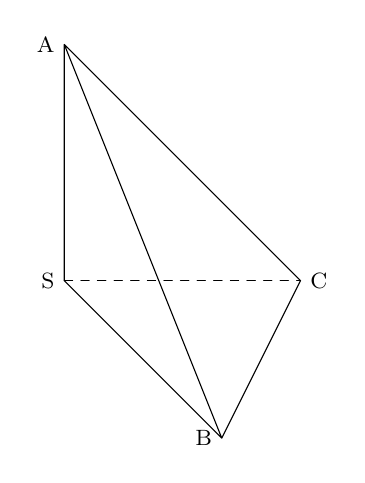
\begin{tikzpicture}[scale=1, font=\footnotesize, line join=round, line cap=round, >=stealth]
				\path 
				(0,0) coordinate[label=left : S] (S)
				(3,0) coordinate[label=right : C] (C)
				(2,-2)coordinate[label=left : B] (B)
				(0,3) coordinate[label=left : A] (A)				;
				\draw (A)--(S)--(B)--(C)--cycle (A)--(B);
				\draw[dashed] (S)--(C);
			\end{tikzpicture}
		\end{center}
		 
		 Ta có $\heva{&SB \perp SA \\& SC \perp SA}$
		 
		 Do đó $\left[B,SA,C\right]=\widehat{CSB}=90^{\circ}$
	}
\end{ex}

%%%==============EX_5============%%%
%\begin{ex}%[1H8H6-1]
%	\immini{	Cho hình chóp $S.ABC$. Hình chiếu vuông góc của $S$ lên $\left(ABC\right)$ trùng với trung điểm $H$ của cạnh $BC$. Biết tam giác $SBC$ là tam giác đều.
%		
%		Tính số đo của góc giữa $SC$ và $\left(ABC\right)$.
%		\choice
%		{\True $60^\circ$}
%		{$75^\circ$}
%		{$45^\circ$}
%		{$30^\circ$}
%		\loigiai{
%			Từ giả thiết ta có $SH\perp \left(ABC\right)$ suy ra $HC$ là hình chiếu của $SC$ trên mặt phẳng $\left(ABC\right)$. 
%			
%			Do đó $\widehat{\left(SC,\left(ABC\right)\right)}=\widehat{\left(SC,HC\right)}=\widehat{SCH}=60^\circ$ (Do tam giác $SBC$ là tam giác đều).
%	}}{
%		\begin{tikzpicture}[scale=1, font=\footnotesize, line join=round, line cap=round, >=stealth]
%			\draw[dashed] (0,0)--(4,0)--(1,-1);
%			\draw(0,0)--(2,-2)--(4,0)--(1,4)--(1,-1) (0,0)--(1,4)--(2,-2);
%			\node[right] at (4,0) {$A$} ;
%			\node[left] at (0,0) {$B$} ;
%			\node[below left]at (2,-2) {$C$} ;
%			\node[left]at (1,4) {$S$} ;
%			\node[left]at (1,-1) {$H$} ;
%		\end{tikzpicture}
%	}
%\end{ex}
%%%==============EX_6============%%%
\begin{ex}%[1H8V6-2]
	Cho hình chóp $S.ABCD$ có đáy $ABCD$ là hình chữ nhật tâm $O$, $SA\perp \left(ABCD\right)$. Gọi $H$ là hình chiếu của $S$ lên $BD$. Góc phẳng nhị diện $\left[S, BD, A\right]$ là
	\choice
	{$\widehat{SOA}$}
	{$\widehat{SBA}$}
	{\True $\widehat{SHA}$}
	{$\widehat{SDA}$}
	\loigiai{ \immini{
			Ta có $SH\perp BD$ và $AH\perp BD$ suy ra $\widehat{SHA}$ là góc phẳng nhị diện $\left[S, BD, A\right]$.}
		{
			\begin{tikzpicture}
				\path
				(0,3) coordinate[label=left: S] (S)
				(0,0) coordinate[label=left: A] (A)
				(2,-1) coordinate[label=right: C] (C)
				(4,0) coordinate[label=right: D] (D)
				(-2,-1) coordinate[label=left: B] (B)
				($(B)!.4!(D)$) coordinate[label=below: H] (H)
				($(B)!.5!(D)$)  coordinate[label=below: O] (O);
				\draw (D)--(C)--(B);
				\draw[dashed] (B)--(A)--(D);
				\draw[dashed] (A)--(C) (D)--(B);
				\draw[dashed] (O)--(S)--(A);
				\draw (B)--(S)--(C)  (D)--(S);
				\draw[dashed] (A)--(H)--(S) ;
				
			\end{tikzpicture}
		}
	}
\end{ex}
%%%==============EX_7============%%%
\begin{ex}%[1H8N6-2]
	Cho hình lăng trụ đứng $ABC.A'B'C'$ có đáy $ABC$ là tam giác vuông tại $A$. Góc phẳng nhị diện $\left[B, AA', C\right]$ có số đo bằng
	\choice
	{$30^\circ$}
	{$45^\circ$}
	{$60^\circ$}
	{\True $90^\circ$}
	\loigiai{ \immini{
			Ta có $BA\perp AA'$ và $CA\perp AA'$ suy ra $\widehat{BAC}$ là góc phẳng nhị diện $\left[B, AA', C\right]$ và bằng $90^\circ$.}
		{
			{
				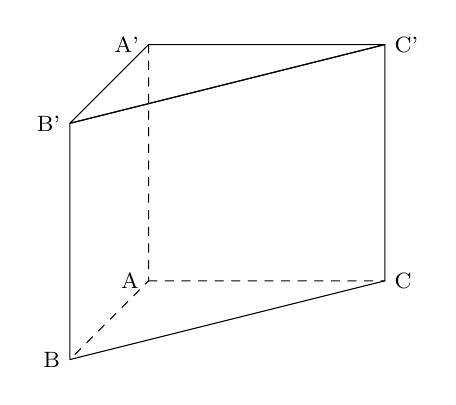
\begin{tikzpicture}[scale=1, font=\footnotesize, line join=round, line cap=round, >=stealth]
					\path
					(0,3) coordinate[label=left: A'] (A')
					(0,0) coordinate[label=left: A] (A)
					(3,0) coordinate[label=right: C] (C)
					(3,3) coordinate[label=right: C'] (C')
					(-1,2) coordinate[label=left: B'] (B')
					(-1,-1) coordinate[label=left: B] (B);
					\draw (A')--(B')--(C')--cycle;
					\draw (B)--(B')--(C')--(C)--cycle;
					\draw[dashed] (A')--(A)--(B) (A)--(C) ;		
				\end{tikzpicture}
			}
		}
	}
\end{ex}

%%%==============EX_8============%%%
\begin{ex}%[1H8V6-1]
	Cho hình lập phương $ABCD.A'B'C'D'$, gọi $H$ là hình chiếu của $B$ lên $A'C$. Góc phẳng nhị diện $\left[B, A'C, D\right]$ là
	\choice
	{\True $\widehat{BHD}$}
	{$\widehat{BCD}$}
	{$\widehat{BA'D}$}
	{$\widehat{BAD}$}
	\loigiai{\immini{
			Ta có $BH\perp A'C$ và $DH\perp A'C$ suy ra $\widehat{BHD}$  là góc phẳng nhị diện $\left[B, A'C, D\right]$.}
		{
			\begin{tikzpicture}[scale=1, font=\footnotesize, line join=round, line cap=round, >=stealth]
				\path 
				(0,0) coordinate[label=left: A] (A)
				(5,0) coordinate[label=right: D] (D)
				(3,-2) coordinate[label=right: C] (C)
				(-2,-2) coordinate[label=left: B] (B)
				(0,5) coordinate[label=left: A'] (A')
				(5,5) coordinate[label=right: D'] (D')
				(3,3) coordinate[label=right: C'] (C')
				(-2,3) coordinate[label=left: B'] (B')
				($(A')!0.6!(C)$) coordinate[label=left: H] (H)
				;
				\draw (A')--(B')--(C')--(D')--cycle  (B')--(B)--(C)--(D)--(D') (C)--(C');
				\draw[dashed] (A')--(A)--(B) (A)--(D)  (A')--(C) (B)--(H)--(D) ;
				
			\end{tikzpicture}
		}
	}
\end{ex}

%%%==============EX_9============%%%
%\begin{ex}%[1H8H6-1]
%	\immini{	Cho hình chóp $S.ABCD$ đáy $ABCD$ là hình vuông, cạnh bên $SA$ vuông góc với đáy, $SA=a\sqrt{3}$, $AB=a$. Tính góc giữa đường thẳng $SD$ và mặt phẳng $\left(SAB\right)$.
%		\choice
%		{\True $30^\circ$}
%		{$60^\circ$}
%		{$45^\circ$}
%		{$90^\circ$}
%		\loigiai{
%			Ta có $AD\perp AB.$ $ \quad (1)$
%			
%			Mặt khác $SA\perp \left(ABCD\right)$.
%			
%			$\Rightarrow SA\perp AD$. $ \quad (2)$
%			
%			Từ $(1)$ và $(2)$ $\Rightarrow AD\perp \left(SAB\right)$.
%			
%			$\Rightarrow SA$ là hình chiếu của $SD$ lên $\left(SAB\right)$.
%			
%			$\Rightarrow \widehat{\left(SD,\left(SAB\right)\right)}=\widehat{\left(SD,SA\right)}=\widehat{DSA}$.
%			
%			Ta có $\triangle SAD$ vuông tại $A$.
%			
%			$\Rightarrow \tan \widehat{DSA}=\dfrac{AD}{SA}=\dfrac{1}{\sqrt{3}} \Rightarrow \widehat{DSA}=30^\circ$.
%	}}
%	{
%		\begin{tikzpicture}
%			\path
%			(0,3) coordinate[label=left: S] (S)
%			(0,0) coordinate[label=left: A] (A)
%			(2,-1) coordinate[label=right: C] (C)
%			(4,0) coordinate[label=right: D] (D)
%			(-2,-1) coordinate[label=left: B] (B);
%			\draw (D)--(C)--(B);
%			\draw[dashed] (B)--(A)--(D);
%			\draw[dashed] (S)--(A);
%			\draw (B)--(S)--(C)  (D)--(S);
%		\end{tikzpicture}
%	}
%\end{ex}
%%%==============EX_10============%%%
\begin{ex}%[1H8N6-2]
	Trong các khẳng định sau, khẳng định nào đúng?
	\choice
	{Các góc phẳng nhị diện của một góc nhị diện có số đo phụ thuộc vào vị trí của đỉnh góc}
	{Số đo góc nhị diện không vượt quá $90^{\circ}$}
	{\True Góc phẳng nhị diện của góc nhị diện là góc có đỉnh nằm trên cạnh của góc nhị diện, hai cạnh lần lượt nằm trên hai mặt của nhị diện và vuông góc với cạnh của nhị diện}
	{Góc nhị diện chính là góc giữa hai mặt phẳng}
	\loigiai{
	}
\end{ex}

%%%==============EX_11============%%%
\begin{ex}%[1H8H6-1]
	Cho tam giác $ABC$ vuông cân tại $A$ và $BC=a$. Trên đường thẳng qua $A$ vuông góc với $\left(ABC\right)$ lấy điểm $S$ sao cho $SA=\dfrac{a\sqrt{6}}{2}$. Tính số đo giữa đường thẳng $SB$ và $\left(SAC\right)$.
	\choice
	{\True $30^\circ$}
	{$60^\circ$}
	{$45^\circ$}
	{$90^\circ$}
	\loigiai{\immini{
			Có $\heva{&AB\perp SA \\ &AB\perp AC}$
			
			$\Rightarrow AB\perp \left(SAC\right)$, suy ra $SA$ là hình chiếu vuông góc của $SB$ trên $\left(SAC\right)$.
			
			Vì tam giác $SAB$ vuông tại $A$ nên $\widehat{BSA}$ nhọn.
			
			Suy ra góc giữa $SB$ và $\left(SAC\right)$ bằng góc giữa $SB$ và $SA$ và bằng $\widehat{BSA}$.
			
			Tam giác $ABC$ vuông cân tại $A$, suy ra $AB=\dfrac{BC}{\sqrt{2}}=\dfrac{a}{\sqrt{2}}$.
			
			Có $\tan \widehat{BSA}=\dfrac{AB}{SA}=\dfrac{1}{\sqrt{3}} \Rightarrow \widehat{BSA}=30^\circ$.}
		{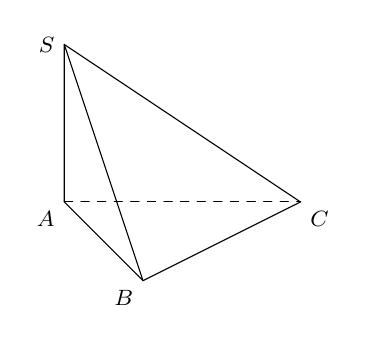
\begin{tikzpicture}[scale=1, font=\footnotesize, line join=round, line cap=round, >=stealth]
				\draw (0,0)--(1,-1)--(3,0)--(0,2)--cycle;
				\draw[dashed] (0,0)--(3,0);
				\draw (0,2)--(1,-1);
				\node[below left] at (0,0) {$A$} ;
				\node[below left]at (1,-1) {$B$} ;
				\node[below right]at (3,0) {$C$} ;
				\node[left]at (0,2) {$S$} ;
		\end{tikzpicture}}
	}
\end{ex}

%%%==============EX_12============%%%
\begin{ex}%[1H8H6-1]
	Cho hình chóp $S.ABCD$, đáy $ABCD$ là hình vuông cạnh bằng $a$ và $SA\perp \left(ABCD\right)$. Biết $SA=a\sqrt{2}$. Tính góc giữa $SC$ và $\left(SAB\right)$.
	\choice
	{\True $30^\circ$}
	{$45^\circ$}
	{$60^\circ$}
	{$75^\circ$}
	\loigiai{\immini{
			Ta có $SA\perp \left(ABCD\right)$
			$\Rightarrow SA\perp BC$.
			
			
			$ABCD$ là hình vuông 
			$\Rightarrow AB\perp BC$.
			
			Do đó $BC\perp \left(SAB\right)$.
			
			$\Rightarrow \widehat{\left(SC,\left(SAB\right)\right)}=\widehat{\left(SC,SB\right)}=\widehat{CSB}$.
			
			Ta có $\triangle SAB$ vuông, suy ra
			\begin{align*}
			SB&=\sqrt{SA^2+AB^2}\\
			&=\sqrt{\left(a\sqrt{2} \right)^2+a^2}=a\sqrt{3}.
			\end{align*}
		
			
			$\Rightarrow \tan \widehat{CSB}=\dfrac{BC}{SB}=\dfrac{\sqrt{3}}{3} \Rightarrow \alpha=30^\circ$.}
		{
			\begin{tikzpicture}[scale=1, font=\footnotesize, line join=round, line cap=round, >=stealth]
				\path
				(0,3) coordinate[label=left: S] (S)
				(0,0) coordinate[label=left: A] (A)
				(2,-1) coordinate[label=right: C] (C)
				(4,0) coordinate[label=right: D] (D)
				(-2,-1) coordinate[label=left: B] (B)
				($(B)!.5!(D)$)  coordinate[label=below: O] (O);
				\draw (D)--(C)--(B);
				\draw[dashed] (B)--(A)--(D);
				\draw[dashed] (A)--(C) (D)--(B);
				\draw[dashed] (O)--(S)--(A);
				\draw (B)--(S)--(C)  (D)--(S);
				\draw[dashed] (A)--(S) ;
				
			\end{tikzpicture}
		}
	}
\end{ex}

\Closesolutionfile{ans}
\indapan{6}{ans/ans-d1-lc}

\cauds
\Opensolutionfile{ans}[ans/ans-d1-ds]
%%%%==============Cau_EX1==============%%%
\begin{ex}%[1H8V6-5]
	Cho hình chóp $S.ABCD$ có đáy là hình vuông cạnh $a$. Biết $SA$ vuông góc với mặt phẳng đáy và $SA=a\sqrt{3}$.  Vẽ đường cao $AH$ của tam giác $SAB$. Vẽ đường cao $AK$ của tam giác $SAD$. Khi đó, các mệnh đề sau \textbf{ĐÚNG} hay \textbf{SAI} ?
	\choiceTF
	{\True $BC\perp AH$}
	{\True Khoảng cách từ $A$ đến mặt phẳng $(SBC)$ bằng $\dfrac{a\sqrt{3}}{2}$}
	{Khoảng cách từ $A$ đến mặt phẳng $(SBD)$ bằng $\dfrac{a\sqrt{2}}{7}$}
	{Khoảng cách từ $C$ đến mặt phẳng $(AHK)$ bằng $\dfrac{a\sqrt{5}}{5}$}
	\loigiai{
		
		
\begin{center}
				\begin{tikzpicture}[scale=1, font=\footnotesize, line join=round, line cap=round, >=stealth]
		\path
		(0,3) coordinate[label=left: S] (S)
		(0,0) coordinate[label=left: A] (A)
		(2,-1) coordinate[label=right: C] (C)
		(4,0) coordinate[label=right: D] (D)
		(-2,-1) coordinate[label=left: B] (B)
		($(B)!.5!(D)$)  coordinate[label=below: O] (O)
		($(B)!.4!(S)$)  coordinate[label=below: H] (H)
		($(D)!.4!(S)$)  coordinate[label=below: K] (K);
		\draw (D)--(C)--(B);
		\draw[dashed] (B)--(A)--(D);
		\draw[dashed] (A)--(C) (D)--(B);
		\draw[dashed] (S)--(A);
		\draw (B)--(S)--(C)  (D)--(S);
		\draw[dashed] (A)--(K) (A)--(H);
		\draw[dashed] (A)--(S) ;
		
	\end{tikzpicture}
\end{center}
	
	\begin{itemchoice}
			\itemch Đúng.
			
			Ta có $\heva{&BC\perp SA(\text{do} SA\perp (ABCD) \\ &BC\perp AB} \Rightarrow BC\perp (SAB)\Rightarrow BC\perp AH$
			\itemch Đúng.
			
			Ta có $BC\perp AH$ mà $SB\perp AH$ nên $AH\perp (SBC)$ hay $\mathrm{d}(A,(SBC))=AH$.
			
			Tam giác $SAB$ vuông tại $A$ có đường cao $AH$ nên
			\[\dfrac{1}{AH^2}=\dfrac{1}{AB^2}+\dfrac{1}{SA^2} \Rightarrow AH=\dfrac{AB\cdot SA}{\sqrt{AB^2+SA^2}}=\dfrac{a\cdot a\sqrt{3}}{\sqrt{a^2+3a^2}}=\dfrac{a\sqrt{3}}{2}.\]
			
			Vậy $\mathrm{d}(A,(SBC))=AH=\dfrac{a\sqrt{3}}{2}$.
			
			
			\itemch Sai.
			
				Gọi $O$ là tâm hình vuông $ABCD$ thì $AO\perp BD$.
			
			 Ta lại có $SA\perp BD$ nên $BD\perp (SAC).$ $ \qquad (*)$
			
			Kẻ đường cao $AE$ của $\triangle SAO$ thì $AE\perp BD$ (do $(*)$).
			
			Vậy $AE\perp (SBD)$ hay $\mathrm{d}(A,(SBD)=AE$.
			
			Ta có $AC=a\sqrt{2}$ (đường chéo hình vuông), suy ra $OA=\dfrac{AC}{2}=\dfrac{a\sqrt{2}}{2}$.
			
			Tam giác $SAO$ vuông tại $A$ có $AE=\dfrac{SA\cdot AO}{\sqrt{SA^2+AO^2}}=\dfrac{a\sqrt{3} \cdot \dfrac{a\sqrt{2}}{2}}{\sqrt{3a^2+\dfrac{2a^2}{4}}}=\dfrac{a\sqrt{21}}{7}$.
			
			Vậy $d(A,(SBD))=AE=\dfrac{a\sqrt{21}}{7}$.
			\itemch Sai.
			
				Ta chứng minh được $AK\perp (SCD)$. Khi đó: $\heva {&SC\perp AH \\ &SC\perp AK} \Rightarrow SC\perp (AHK)$.
			
			Gọi $F=SC\cap (AHK)$ thì $SC\perp AF$.
			Khi đó: $\mathrm{d}(C,(AHK))=CF$.
			
			Ta có $SC=\sqrt{SA^2+AC^2}=\sqrt{3a^2+2a^2}=a\sqrt{5}$.
			
			Tam giác $SAC$ vuông tại $A$ có đường cao $AF$ nên:
			\[CF\cdot CS=AC^2\Rightarrow CF=\dfrac{AC^2}{CS}=\dfrac{2a^2}{a\sqrt{5}}=\dfrac{2a\sqrt{5}}{5}.\]
			Vậy $\mathrm{d}(C,(AHK))=CF=\dfrac{2a\sqrt{5}}{5}$
		\end{itemchoice}
	
	}
\end{ex}
%%%%==============HetCau_EX1==============%%%
%%%%==============Cau_EX2==============%%%
\begin{ex}%[1H8V6-5]
	Cho hình chóp $S.ABC$ có mặt bên $(SAB)$ vuông góc với mặt đáy và tam giác $SAB$ đều cạnh $2a$. Biết tam giác $ABC$ vuông tại $C$ và cạnh $AC=a\sqrt{3}$. Khi đó, các mệnh đề sau \textbf{ĐÚNG} hay \textbf{SAI} ?
	\choiceTF
	{\True $SH\perp (ABC)$}
	{\True $\mathrm{d}(S,(ABC))=a\sqrt{3}$}
	{$\mathrm{d}(C,(SAB))=\dfrac{a\sqrt{3}}{3}$}
	{Thể tích của khối chóp $S.ABC$ bằng $\dfrac{a^3}{6}$}
	\loigiai{
		
		\begin{center}
				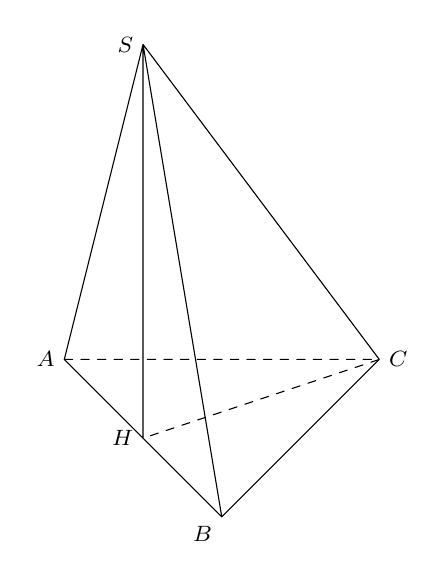
\begin{tikzpicture}[scale=1, font=\footnotesize, line join=round, line cap=round, >=stealth]
			\draw[dashed] (0,0)--(4,0)--(1,-1);
			\draw(0,0)--(2,-2)--(4,0)--(1,4)--(1,-1) (0,0)--(1,4)--(2,-2);
			\node[right] at (4,0) {$C$} ;
			\node[left] at (0,0) {$A$} ;
			\node[below left]at (2,-2) {$B$} ;
			\node[left]at (1,4) {$S$} ;
			\node[left]at (1,-1) {$H$} ;
		\end{tikzpicture}
		\end{center}
		
		\begin{itemchoice}
			\itemch Đúng.
			
			Gọi $H$ là trung điểm $AB$, mà tam giác $SAB$ đều nên $SH\perp AB$.
			
			Ngoài ra $(SAB)\perp (ABC)$ nên $SH\perp (ABC)$.
			\itemch Đúng.
			
				Ta có $\mathrm{d}(S,(ABC))=SH=\dfrac{2a\cdot \sqrt{3}}{2}=a\sqrt{3}$ ( do tam giác $SAB$ đều cạnh $2a$).
			\itemch Sai.
			
			Kẻ đường cao $CK$ của tam giác $ABC$.
			
			Ta có $\heva{&CK\perp AB\\ &CK\perp SH} \Rightarrow CK\perp (SAB)\Rightarrow \mathrm{d}(C,(SAB))=CK$.
	
			Xét tam giác $ABC$ vuông tại $C$ có
			\[BC=\sqrt{AB^2-AC^2}=\sqrt{4a^2-3a^2}=a;CK=\dfrac{CA\cdot CB}{AB}=\dfrac{a\sqrt{3} \cdot a}{2a}=\dfrac{a\sqrt{3}}{2}.\]
			
			Vậy $\mathrm{d}(C,(SAB))=CK=\dfrac{a\sqrt{3}}{2}$.
			\itemch Sai.
			
			Diện tích đáy hình chóp là: $S_{\triangle ABC}=\dfrac{1}{2} AC\cdot BC=\dfrac{1}{2} a\sqrt{3} \cdot a=\dfrac{a^2\sqrt{3}}{2}$.
			
			Thể tích khối chóp là: $V_{S. ABC}=\dfrac{1}{3} SH\cdot S_{\triangle ABC}=\dfrac{1}{3} \cdot a\sqrt{3} \cdot \dfrac{a^2\sqrt{3}}{2}=\dfrac{a^3}{2}$
		\end{itemchoice}
	}
\end{ex}
%%%%==============HetCau_EX2==============%%%

%%%%==============Cau_EX3==============%%%
\begin{ex}%[1H8V6-6]
	Cho lăng trụ đứng $ABC.A' B' C'$ có $AC=a$, $BC=2a$, $\widehat{ACB}=120^{\circ}$. Gọi $M$ là trung điểm của $BB'$. Khi đó, các mệnh đề sau \textbf{ĐÚNG} hay \textbf{SAI} ?
	\choiceTF
	{\True $\mathrm{d}\left(CC', \left(ABB' A' \right)\right)=\dfrac{a\sqrt{21}}{7}$}
	{$\mathrm{d}\left(CC', AM\right)=\dfrac{a\sqrt{21}}{12}$}
	{\True $AA' \perp (ABC)$, $AA' \perp \left(A' B' C' \right)$}
	{\True Biết khoảng cách giữa hai mặt đáy lăng trụ bằng $2a$. Khi đó thể tích khối lăng trụ là $a^3\sqrt{3}$}
	\loigiai{
		
		\begin{center}
				\begin{tikzpicture}[scale=1, font=\footnotesize, line join=round, line cap=round, >=stealth]
			\path
			(0,3) coordinate[label=left: A'] (A')
			(0,0) coordinate[label=above right: A] (A)
			(3,0) coordinate[label=right: C] (C)
			(3,3) coordinate[label=right: C'] (C')
			(-1,2) coordinate[label=left: B'] (B')
			(-1,-1) coordinate[label=left: B] (B)
			($(B)!.5!(B')$) coordinate[label=left: M] (M);
			\draw (A')--(B')--(C')--cycle;
			\draw (B)--(B')--(C')--(C)--cycle;
			\draw[dashed] (A')--(A)--(B) (A)--(C) ;		
			\draw[dashed] (M)--(A);
		\end{tikzpicture}
		\end{center}
		
		\begin{itemchoice}
			\itemch 	Đúng.
			
				Ta có $CC' \parallel BB' \Rightarrow CC' \parallel \left(ABB' A' \right)$ nên $d\left(CC', \left(ABB' A' \right)\right)=\mathrm{d}\left(C,\left(ABB' A' \right)\right)$.
			
			Trong mặt phẳng $(ABC)$, kẻ $CH\perp AB$ tại $H$.  $\quad (1)$
			
			Vì $ABC.A' B' C'$ là hình lăng trụ đứng nên $AA' \perp (ABC) \Rightarrow CH\perp AA'$. (2)
			
			
			Từ (1) và (2) suy ra $CH\perp \left(ABB' A' \right)\Rightarrow \mathrm{d}\left(C,\left(ABB' A' \right)\right)=CH$.
			
			Xét tam giác $ABC$, có $AB^2=CA^2+CB^2-2CA\cdot CB\cdot \cos 120^{\circ}=7a^2$ $\Rightarrow AB=a\sqrt{7}$.
			
			Diện tích tam giác $ABC$ là $S_{\triangle ABC}=\dfrac{1}{2} CA\cdot CB\cdot \sin C=\dfrac{1}{2} AB\cdot CH$ 
			
			$\Rightarrow CH=\dfrac{CA\cdot CB\cdot \sin 120^{\circ}}{AB}=\dfrac{a\cdot 2a\cdot \dfrac{\sqrt{3}}{2}}{a\sqrt{7}}=\dfrac{a\sqrt{21}}{7}$.
			
			Vậy $\mathrm{d}\left(CC', \left(ABB' A' \right)\right)=CH=\dfrac{a\sqrt{21}}{7}$.
			
				\itemch Sai.
				
				Ta có $AM$ và $CC'$ là hai đường thẳng chéo nhau mà $\heva{&CC' \parallel \left(ABB' A' \right) \\ &AM\subset \left(ABB' A' \right)}$
			nên $\mathrm{d}\left(CC', AM\right)=\mathrm{d}\left(CC', \left(ABB' A' \right)\right)=\dfrac{a\sqrt{21}}{7}$.
		
			
		\itemch Đúng.
		
			Vì $ABC. A' B' C'$ là hình lăng trụ đứng nên $AA' \perp (ABC)$, $AA' \perp \left(A' B' C' \right)$.
			
			
				Do vậy $\mathrm{d}\left((ABC),\left(A' B' C' \right)\right)=AA'=2a$.
			
			\itemch Đúng.
			
			Khối lăng trụ $ABC.A' B' C'$ có chiều cao $h=AA'=2a$, diện tích đáy là:
			\[S=S_{ABC}=\dfrac{1}{2} CA\cdot CB\cdot \sin 120^{\circ}=\dfrac{1}{2} a\cdot 2a\cdot \dfrac{\sqrt{3}}{2}=\dfrac{a^2\sqrt{3}}{2}.\]
			
			Thể tích khối lăng trụ là: $V=Sh=\dfrac{a^2\sqrt{3}}{2} \cdot 2a=a^3\sqrt{3}$.
		\end{itemchoice}
	}
\end{ex}
%%%%==============HetCau_EX3==============%%%
%%%%==============Cau_EX4==============%%%
\begin{ex}%[1H8V6-5]
	Cho hình chóp $S.ABC$ có đáy là tam giác $ABC$ vuông tại $B$ có $AB=1$,\quad \, \(\widehat{ACB}=30^{\circ}\). Biết $SA$ vuông góc với mặt đáy và $SA=2$. Gọi $H$ là hình chiếu của $A$ trên $SB$. Khi đó, các mệnh đề sau \textbf{ĐÚNG} hay \textbf{SAI} ?
	\choiceTF
	{\True $\mathrm{d}(A,SB)=AH$}
	{$\mathrm{d}(B,(SAC))=\dfrac{\sqrt{3}}{3}$}
	{\True $BC=\sqrt{3}$}
	{Thể tích khối chóp $S.ABC$ bằng $\dfrac{\sqrt{3}}{6}$}
	\loigiai{
		
	\begin{center}
			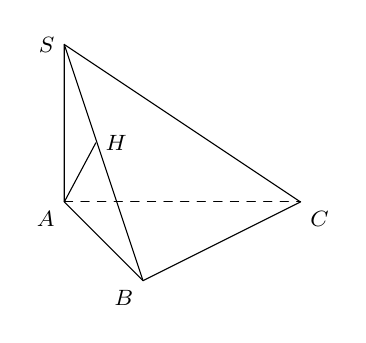
\begin{tikzpicture}[scale=1, font=\footnotesize, line join=round, line cap=round, >=stealth]
			\draw (0,0)--(1,-1)--(3,0)--(0,2)--cycle (0,0)--(.4,0.75);
			\draw[dashed] (0,0)--(3,0);
			\draw (0,2)--(1,-1);
			\node[below left] at (0,0) {$A$} ;
			\node[below left]at (1,-1) {$B$} ;
			\node[below right]at (3,0) {$C$} ;
			\node[left]at (0,2) {$S$} ;
			\node[right]at (0.4,0.75) {$H$} ;
		\end{tikzpicture}
	\end{center}
		
		\begin{itemchoice}
			\itemch Đúng.
			
			Vì $AH\perp SB$ nên $\mathrm{d}(A,SB)=AH$. 
			
			Tam giác $SAB$ vuông tại $A$, đường cao $AH$ nên $\dfrac{1}{AH^2}=\dfrac{1}{SA^2}+\dfrac{1}{AB^2}$
			\[\Rightarrow AH=\dfrac{SA\cdot AB}{\sqrt{SA^2+AB^2}}=\dfrac{2\cdot 1}{\sqrt{2^2+1^2}}=\dfrac{2\sqrt{5}}{5}.\]
			\itemch Sai.
			
			Trong mặt phẳng $(ABC)$, kẻ $BI\perp AC$ tại $I$.
			
			Mặt khác $BI\perp SA$ (do $SA\perp (ABC)$, $BI\subset (ABC)$.
			
			Vì vậy $BI\perp (SAC)$ hay $d(B,(SAC)=BI$.
			
			Tam giác $ABI$ vuông tại $I$ có $\sin \widehat{BAC}=\dfrac{BI}{AB}$ $\Rightarrow BI=AB\cdot \sin 60^{\circ}=\dfrac{\sqrt{3}}{2}$.
			
			Vậy $\mathrm{d}(B,(SAC))=BI=\dfrac{\sqrt{3}}{2}$.
			\itemch  Đúng.
			
			Tam giác $ABC$ vuông tại $B$ có $\tan \widehat{ACB}=\dfrac{AB}{BC}$ $\Rightarrow BC=\dfrac{AB}{\tan 30^{\circ}}=\sqrt{3}$.
			\itemch Sai.
			
		Diện tích đáy hình chóp là $S=S_{\triangle ABC}=\dfrac{1}{2} BA \cdot BC=\dfrac{\sqrt{3}}{2}$. 
			
			Chiều cao hình chóp $h=SA=2$.
			
			Thể tích khối chóp $S.ABC$ là: $V_{S.ABC}=\dfrac{1}{3} Sh=\dfrac{1}{3} \cdot \dfrac{\sqrt{3}}{2} \cdot 2=\dfrac{\sqrt{3}}{3}$ (đơn vị thể tích).
		\end{itemchoice}
	}
\end{ex}
%%%%==============HetCau_EX4==============%%%

\Closesolutionfile{ans}
\indapan{3}{ans/ans-d1-ds}

\Opensolutionfile{ans}[ans/ans-d1-kq]
\caukq
%%%==============BT_1==============%%%
\begin{bt}%[1H8V6-7]
	Kim tự tháp Memphis tại bang Tennessee (Mỹ) có dạng hình chóp tứ giác đều với chiều cao $98$ m và cạnh đáy $180$ m. Tính số đo góc nhị diện tạo bởi mặt bên và mặt đáy của kim tự tháp đó. (đơn vị đo góc là độ, làm tròn đến hàng phần chục)
	\shortans{$47{,}4$}
	\loigiai{
		
	\begin{center}
				\begin{tikzpicture}
				\path 
				(0,0) coordinate[label=left: A] (A)
				(-1,-1) coordinate[label=left: B] (B)
				(3,0) coordinate[label=right: D] (D)
				(2,-1) coordinate[label=right: C] (C)
				(1,3) coordinate[label=left: S] (S)
				($(A)!0.5!(C)$) coordinate[label=below: O] (O)
				;
			\draw (D)--(C)--(B);
			\draw[dashed] (B)--(A)--(D);
			\draw[dashed] (A)--(C) (D)--(B);
			\draw[dashed] (S)--(A);
			\draw (B)--(S)--(C)  (D)--(S);


		\end{tikzpicture}
	\end{center}
		Xét hình chóp tứ giác đều $S.ABCD$ có chiều cao $98$ m và cạnh đáy $180$ m\\
		Gọi $O$ là tâm hình vuông $ABCD$ thì $SO\perp (ABCD)\Rightarrow SO\perp AB$. $ \qquad (1)$\\
		Gọi $M$ là trung điểm $AB$ thì $OM$ là đường trung bình của tam giác $ABC$, \\
		Suy ra $OM=\dfrac{BC}{2}=90$ (m) và $OM\perp AB.$ $\qquad (2)$\\
		Từ $(1)$ và $(2)$ suy ra $\widehat{SMO}$ là góc phẳng nhị diện $[S,AB,O]$ \\
		với $$\tan \widehat{SMO}=\dfrac{SO}{OM}=\dfrac{98}{90}=\dfrac{49}{45} \Rightarrow \widehat{SMO}\approx 47{,}44^{\circ}$$
		Vậy góc nhị diện tạo bởi mặt bên và mặt đáy của kim tự tháp xấp xỉ $47{,}44^{\circ}$.
	}
\end{bt}

%%%==============BT_2==============%%%
\begin{bt}%[1H8V6-2]
	Cho hình chóp $S.ABCD$ có đáy là hình vuông cạnh $a$ và $SA\perp (ABCD)$. Biết góc giữa $SC$ và mặt phẳng $(ABCD)$ là $60^{\circ}$. Tính góc phẳng nhị diện $[S,BD,C]$?(đơn vị đo góc là độ, làm tròn đến hàng đơn vị)
	\shortans{ $106$}
	\loigiai{
		
\begin{center}
						\begin{tikzpicture}[scale=1, font=\footnotesize, line join=round, line cap=round, >=stealth]
			\path
			(0,3) coordinate[label=left: S] (S)
			(0,0) coordinate[label=left: A] (A)
			(2,-1) coordinate[label=right: C] (C)
			(4,0) coordinate[label=right: D] (D)
			(-2,-1) coordinate[label=left: B] (B)
			($(B)!.5!(D)$)  coordinate[label=below: O] (O);
			\draw (D)--(C)--(B);
			\draw[dashed] (B)--(A)--(D);
			\draw[dashed] (A)--(C) (D)--(B);
			\draw (B)--(S)--(C)  (D)--(S);
			\draw[dashed] (A)--(S) ;
			
		\end{tikzpicture}
\end{center}
		
		Ta có $SA\perp (ABCD)$ tại $A$ và $SC$ cắt mp $(ABCD)$ tại $C$.\\
		$\Rightarrow AC$ là hình chiếu của $SC$ trên mp $(ABCD)$.\\
		$\Rightarrow (SC,(ABCD))=(SC,AC)=\widehat{SCA}=60^{\circ}
		$.\\
		 $\Rightarrow SA=AC\cdot \tan 60^{\circ}=a\sqrt{2} \cdot \sqrt{3}=\sqrt{6} a$.\\
		Ta có $\heva{&BD\perp SA \\ &BD\perp AC} \Rightarrow BD\perp (SAC)$.\\
		Ta có $\heva{&(SBD)\cap (CBD)=BD \\
			 &\text{Trong } (CBD),CO\perp BD\\ 
			 &\text{Trong } (SBC),SO\perp BD} 
			 \Rightarrow [S,BD,C]=\widehat{SOC}.$\\
		Xét $\triangle SAO$ vuông tại $A:\tan \widehat{SOA}=\dfrac{SA}{AO}=\dfrac{a\sqrt{6}}{\dfrac{a\sqrt{2}}{2}}=2\sqrt{3} $.\\
		$\Rightarrow \widehat{SOA}=73{,}9^\circ$.\\
		$\Rightarrow \widehat{SOC}=106^\circ
		$.
	}
\end{bt}

%%%==============BT_3==============%%%
\begin{bt}%[1H8H6-5]
	Cho hình hộp chữ nhật $ABCD.A' B' C' D'$ có $AB=a$, $AD=2a$, $AA'=3a$. Tính góc phẳng nhị diện $\left[A',BD,A\right]$? (đơn vị đo góc là độ, làm tròn đến hàng phần chục)
	\shortans{$73{,}4$}
	\loigiai{
		
		\begin{center}
				\begin{tikzpicture}[scale=1, font=\footnotesize, line join=round, line cap=round, >=stealth]
				\path 
				(0,0) coordinate[label=left: A] (A)
				(5,0) coordinate[label=right: D] (D)
				(3,-2) coordinate[label=right: C] (C)
				(-2,-2) coordinate[label=left: B] (B)
				(0,4) coordinate[label=left: A'] (A')
				(5,4) coordinate[label=right: D'] (D')
				(3,2) coordinate[label=right: C'] (C')
				(-2,2) coordinate[label=left: B'] (B')
				($(B)!.4!(D)$)coordinate[label=below right: I] (I)
				;
				\draw (A')--(B')--(C')--(D')--cycle  (B')--(B)--(C)--(D)--(D') (C)--(C');
				\draw[dashed] (A')--(A)--(B) (A)--(D) (B)--(D) (A)--(I);
				
			\end{tikzpicture}
		\end{center}
		Kẻ $AI\perp BD$.\\
		Mà $BD\perp A' A\Rightarrow BD\perp \left(AA' I\right)$.\\
		Ta có 
		\[\heva{&\left(A' BD\right)\cap (ABD)=BD \\ &\text{Trong }(ABD),AI\perp BD \\ &\text{Trong }\left(A' BD\right),A' I\perp BD} \Rightarrow \left[A', BD,A\right]=\widehat{A {'}IA}.
		\]
		Ta có $AI=\dfrac{1}{\sqrt{\dfrac{1}{AB^2}+\dfrac{1}{AD^2}}}=\dfrac{1}{\sqrt{\dfrac{1}{a^2}+\dfrac{1}{(2a)^2}}}=\dfrac{2\sqrt{5}}{5} a$.\\
		Xét $\Delta AA' I$ vuông tại $A$: $\tan \widehat{A' IA}=\dfrac{A' A}{AI}=\dfrac{3a}{\dfrac{2\sqrt{5}}{5} a}=\dfrac{3\sqrt{5}}{2} \Rightarrow \widehat{A' IA}\approx 73{,}4^{\circ}$.
	}
\end{bt}

%%%==============BT_4==============%%%
\begin{bt}%[1H8C6-2]
	Cho hình chóp $S.ABCD$ có $SA$ vuông góc với đáy $ABCD$, đáy là hình thang vuông tại $A$, có đáy lớn $AB$, $AB=2a$, $AD=DC=a$. Vẽ $AH\perp SC$, $H\in SC$ và $M$ là trung điểm của $AB$. Biết $[S,DC,B]=60^{\circ}$. Gọi $Sx$ là giao tuyến của hai mặt phẳng $(SAD)$ và $(SMC)$. Tính $[A,Sx,M]$? (đơn vị đo góc là độ)
	\shortans{ $30$}
	\loigiai{
		
		\begin{center}
						\begin{tikzpicture}[scale=1, font=\footnotesize, line join=round, line cap=round, >=stealth]
				\path
				(0,3) coordinate[label=left: S] (S)
				(0,0) coordinate[label=left: A] (A)
				(1,-1) coordinate[label=below: C] (C)
				(4,0) coordinate[label=right: B] (B)
				(-1,-1) coordinate[label=left: D] (D)
				($(A)!.5!(B)$) coordinate[label=above right: M] (M)
				($(S)!.4!(C)$) coordinate[label=above right: H] (H)
				;
				\draw (D)--(C)--(B);
				\draw[dashed] (B)--(A)--(D);
				\draw[dashed] (A)--(C) (M)--(S);
				\draw[dashed] (S)--(A)--(H);
				\draw (B)--(S)--(C)  (D)--(S);
				\draw[dashed] (A)--(S) (C)--(M) ;
				
			\end{tikzpicture}
		\end{center}
		Ta có $AD\parallel CM$ (dễ dàng chứng minh được).\\
		Giao tuyến của $(SAD)$ và $(SCM)$:
		\[\begin{array}{l} { \left\{\begin{array}{l} {S\in (SAD)\cap (SCM)} \\ {AD\parallel CM} \\ {AD\subset (SAD),CM\subset (SCM)} \end{array}\right.} \\ {\Rightarrow (SAD)\cap (SCM)=Sx\, \, (Sx \parallel AD \parallel CM)} \end{array}
		\]
		Ta có $DA\perp SA (\text{ do }DA\perp (SAB))$.\\
		$\Rightarrow SA\perp Sx$.\\
		Mà 
		$CM\perp (SAB)$ (vì $CM\parallel AD)\Rightarrow SM\perp CM$\\
		$ \Rightarrow SM\perp Sx$.\\
		Vậy $[A,Sx,M]=\widehat{ASM}$.
		\[\tan \widehat{ASM}=\dfrac{AM}{SA}=\dfrac{a}{a\sqrt{3}}=\dfrac{1}{\sqrt{3}} \Rightarrow \widehat{ASM}=30^{\circ}.
		\]
	}
\end{bt}

%%%==============BT_5==============%%%
\begin{bt}%[1H8H6-2]
	Cho hình chóp $S.ABC$ có đáy là tam giác đều cạnh $a$ và $SA\perp (ABC)$ và $SA=2a$. Tính góc phẳng nhị diện $[A,SC,B]$? (đơn vị đo góc là độ, làm tròn đến hàng phần chục)
	\shortans{$62{,}7$}
	\loigiai{
			\begin{center}
			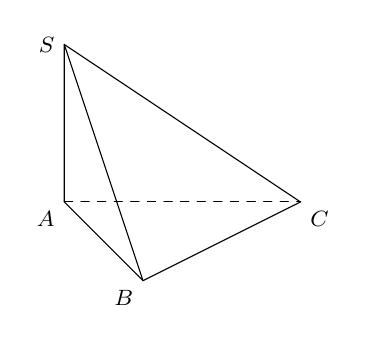
\begin{tikzpicture}[scale=1, font=\footnotesize, line join=round, line cap=round, >=stealth]
				\draw (0,0)--(1,-1)--(3,0)--(0,2)--cycle;
				\draw[dashed] (0,0)--(3,0);
				\draw (0,2)--(1,-1);
				\node[below left] at (0,0) {$A$} ;
				\node[below left]at (1,-1) {$B$} ;
				\node[below right]at (3,0) {$C$} ;
				\node[left]at (0,2) {$S$} ;
			\end{tikzpicture}
		\end{center}
		Kẻ $BI\perp AC$.\\
		Ta có $\heva{&BI\perp AC \\ &BI\perp SA} \Rightarrow BI\perp (SAC)$.\\
		Ta có $\heva{&(SAC)\cap (SBC)=SC \\ &\text{Trong } (SAC),IH\perp SC\Rightarrow [A,SC,B]=\widehat{IHB} \\ & \text{Trong }  (SBC),BH\perp SC}$.\\
		Ta có
		\[\triangle HCI \sim \triangle ACS\Rightarrow \dfrac{HI}{SA}=\dfrac{CI}{SC} \Rightarrow HI=\dfrac{SA\cdot CI}{SC}=\dfrac{2a\cdot \dfrac{a}{2}}{\sqrt{(2a)^2+a^2}}=\dfrac{\sqrt{5}}{5} a.
		\]
		Xét $\Delta BHI$ vuông tại $I:\tan \widehat{BHI}=\dfrac{BI}{HI}=\dfrac{\dfrac{a\sqrt{3}}{2}}{\dfrac{\sqrt{5}}{5} a}=\dfrac{\sqrt{15}}{2} \Rightarrow \widehat{BHI}\approx 62{,}7^\circ$.
	}
\end{bt}

%%%==============BT_6==============%%%
\begin{bt}%[1H8H6-2]
	Cho hình hộp chữ nhật $ABCD\cdot A' B' C' D'$ có $AB=a,AD=2a,AA'=3a$. Tính góc phẳng nhị diện $\left[A', BD,A\right]$? (đơn vị đo góc là độ, làm tròn đến hàng phần chục)
	\shortans{$73{,}4$}
	\loigiai{
		
				\begin{center}
			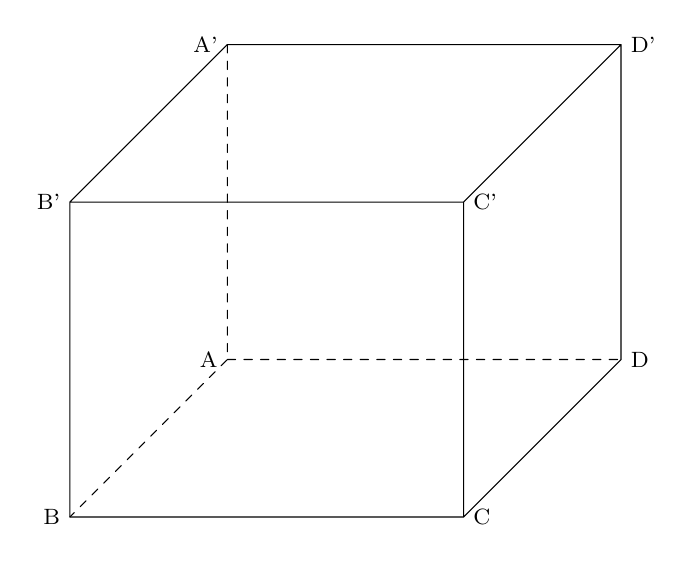
\begin{tikzpicture}[scale=1, font=\footnotesize, line join=round, line cap=round, >=stealth]
				\path 
				(0,0) coordinate[label=left: A] (A)
				(5,0) coordinate[label=right: D] (D)
				(3,-2) coordinate[label=right: C] (C)
				(-2,-2) coordinate[label=left: B] (B)
				(0,4) coordinate[label=left: A'] (A')
				(5,4) coordinate[label=right: D'] (D')
				(3,2) coordinate[label=right: C'] (C')
				(-2,2) coordinate[label=left: B'] (B')
				;
				\draw (A')--(B')--(C')--(D')--cycle  (B')--(B)--(C)--(D)--(D') (C)--(C');
				\draw[dashed] (A')--(A)--(B) (A)--(D);
				
			\end{tikzpicture}
		\end{center}
		Kẻ $AI\perp BD$. \\
		Mà $BD\perp A' A\Rightarrow BD\perp \left(AA' I\right)$.\\
		Ta có
		 $AI=\dfrac{1}{\sqrt{\dfrac{1}{AB^2}+\dfrac{1}{AD^2}}}=\dfrac{1}{\sqrt{\dfrac{1}{a^2}+\dfrac{1}{(2a)^2}}}=\dfrac{2\sqrt{5}}{5} a$.\\
		Xét $\Delta AA' I$ vuông tại $A:\tan \widehat{A' IA}=\dfrac{A' A}{AI}=\dfrac{a\sqrt{3}}{\dfrac{2\sqrt{5}}{5} a}=\dfrac{3\sqrt{5}}{2} \Rightarrow \widehat{A' IA}\approx 73{,}4^{\circ}$.
	}
\end{bt}


\Closesolutionfile{ans}
\indapan{6}{ans/ans-d1-kq}


\newpage
\subsection{Đề 2}
\Opensolutionfile{ans}[ans/ans-d2-lc]
\caulc
%%%==============EX_1============%%%
%\begin{ex}%[1H8N6-1]
%	\immini{	Cho hình chóp $S.ABC$ có $\triangle ABC$ vuông tại $B$ và $SA\perp \left(ABC\right)$. Góc giữa đường thẳng $SC$ và mặt phẳng $\left(SAB\right)$ là góc nào sau đây?
%		\choice
%		{$\widehat{SAC}$}
%		{$\widehat{CSA}$}
%		{\True $\widehat{CSB}$}
%		{$\widehat{SCB}$}
%		\loigiai{ Ta có $\heva{&SA \perp BC\\ &AB \perp BC} \Rightarrow BC \perp (SAB)$
%			
%			Do dó $SB$ là hình chiếu vuông góc của $SC$ lên mặt phẳng $(SAB)$.
%			
%			Vậy $(SC,(SAB))=(SC,SB)=\widehat{CSB}$.
%	}}{\begin{tikzpicture}
%			\draw (0,0)--(1,-1)--(3,0)--(0,2)--cycle;
%			\draw[dashed] (0,0)--(3,0);
%			\draw (0,2)--(1,-1);
%			\node[below left] at (0,0) {$A$} ;
%			\node[below left]at (1,-1) {$B$} ;
%			\node[below right]at (3,0) {$C$} ;
%			\node[left]at (0,2) {$S$} ;
%	\end{tikzpicture}}
%\end{ex}

%%%==============EX_2============%%%
%\begin{ex}%[1H8H6-1]
%	\immini{	Hình chóp $S.ABC$ có đáy $ABC$ là tam giác đều cạnh $a$, mặt phẳng $\left(SAB\right)$ vuông góc với đáy. Biết $\triangle SAB$ là tam giác đều. Hỏi góc giữa đường thẳng $SC$ và mặt phẳng $\left(ABC\right)$ bằng bao nhiêu?
%		\choice
%		{$30^\circ$}
%		{\True $45^\circ$}
%		{$60^\circ$}
%		{$90^\circ$}
%		\loigiai{
%			
%			Gọi $I$ là trung điểm $AB$.
%			
%			Ta có $\heva{&SI \perp AB\\&(SAB) \perp (ABC)\\& (SAB) \cap (ABC)=AB} \Rightarrow SI \perp (ABC)$.\\
%			Do đó $(SC,(ABC))=\widehat{SCI}$.\\
%			Dễ thấy, $\heva{&SI=IC\\&SI \perp IC}$, suy ra tam giác $SIC$ vuông cân tại $I$ .\\
%			Nên $\widehat{SCI}=45^{\circ}$
%	}}{\begin{tikzpicture}
%			\draw[dashed] (0,0)--(2,2)--(5,0) (2,2)--(1,5)--(1,1);
%			\draw (0,0)--(1,5)--(5,0)--cycle;
%			\node[left] at (2,2) {$A$} ;
%			\node[below left]at (0,0) {$B$} ;
%			\node[below right]at (5,0) {$C$} ;
%			\node[left]at (1,5) {$S$} ;
%			\node[left]at (1,1) {$I$} ;
%	\end{tikzpicture}}
%\end{ex}

%%%==============EX_3============%%%
\begin{ex}%[1H8H6-1]
	Cho hình chóp $S.ABCD$ có đáy là hình thoi tâm $O$ cạnh $a$. $\triangle ABC$ cân tại $A$, $SA$ vuông góc với đáy. Tính góc giữa đường thẳng $BC$ với mặt phẳng $\left(SAB\right)$.
	\choice
	{$30^\circ$}
	{$45^\circ$}
	{\True $60^\circ$}
	{$90^\circ$}
	\loigiai{
		\begin{center}
				\begin{tikzpicture}
			\path
			(0,3) coordinate[label=left: S] (S)
			(0,0) coordinate[label=left: A] (A)
			(2,-2) coordinate[label=right: C] (C)
			(4,0) coordinate[label=right: D] (D)
			(-2,-2) coordinate[label=left: B] (B)
			($(A)!0.5!(C)$) coordinate[label=left: O] (O)
			($(A)!0.5!(B)$) coordinate[label=left: H] (H)
			;
			\draw (D)--(C)--(B) ;
			\draw[dashed] (B)--(A)--(D);
			\draw[dashed] (S)--(A) (A)--(C) (B)--(D) (C)--(H)--(S);
			\draw (B)--(S)--(C)  (D)--(S);
		\end{tikzpicture}
		\end{center}
		Ta có tam giác $ABC$ cân tại $A$ và $AB=BC$ (do ABCD là hình thoi).\\
		Nên ta có tam giác $ACB$ là tam giác đều.\\
		Gọi $H$ là trung điểm $AH$. Ta có $\heva{& CH \perp AB\\& CH \perp SA}$ (do $SA \perp (ABCD)$).\\
		Nên $BH$ là hình chiêu vuông góc của $BC$ lên $(SAB)$.\\
		Vậy $(BC, (SAB))=(BC, BH)=\widehat{CBH}=60^{\circ}$ ( do tam giác $ABC$ đều)
	}
\end{ex}

%%%==============EX_4============%%%
\begin{ex}%[1H8N6-2]
	Cho hình chóp $S.ABCD$ có đáy $ABCD$ là hình vuông, $SA$ vuông góc với đáy. Gọi $I$, $J$, $K$ lần lượt là hình chiếu của $A$ lên các cạnh $SB$, $SC$, $SD$. Khi đó góc phẳng nhị diện $\left[I,SA,K\right]$ là góc nào dưới đây?
	\choice
	{$\widehat{IAK}$}
	{$\widehat{ISK}$}
	{\True $\widehat{BAD}$}
	{$\widehat{BSC}$}
	\loigiai{
		
	\begin{center}
				\begin{tikzpicture}
			\path 
			(0,0) coordinate[label=left: A] (A)
			(5,0) coordinate[label=right: D] (D)
			(3,-2) coordinate[label=right: C] (C)
			(-2,-2) coordinate[label=left: B] (B)
			(0,5) coordinate[label=left: S] (S)
			($(S)!0.4!(B)$) coordinate[label=left: I] (I)
			($(S)!0.6!(C)$) coordinate[label=right: J] (J)
			($(S)!0.4!(D)$) coordinate[label=right: K] (K)
			($(S)!0.4!(A)$) coordinate[label=above right: J] (H);
			\draw (S)--(B)--(C)--(D)--cycle  (S)--(C);
			\draw[dashed]  (B)--(A)--(D)  (A)--(S)  (A)--(I) (A)--(J) (I)--(H)--(K) (A)--(K);
		\end{tikzpicture}
	\end{center}
		
		Kẻ $IJ \perp SA$. Do $\triangle SAB = \triangle SAD$ nên $KJ \perp SA$
		
		Nên $\left[I,SA,K\right]=\widehat{IJK}=\widehat{BAD}$ ( Do $AB \parallel IJ $ và $JK \parallel AD$)
	}
\end{ex}

%%%==============EX_5============%%%
\begin{ex}%[1H8H6-2]
	Cho hình lăng trụ đứng $ABC.A'B'C'$ có đáy $ABC$ là tam giác vuông tại $B$, $AB=a\sqrt{3}$, $BC=a$. Góc phẳng nhị diện $\left[B,AA',C\right]$ có số đo
	\choice
	{\True $30^\circ$}
	{$60^\circ$}
	{$120^{\circ}$}
	{$90^\circ$}
	\loigiai{
			\begin{center}
			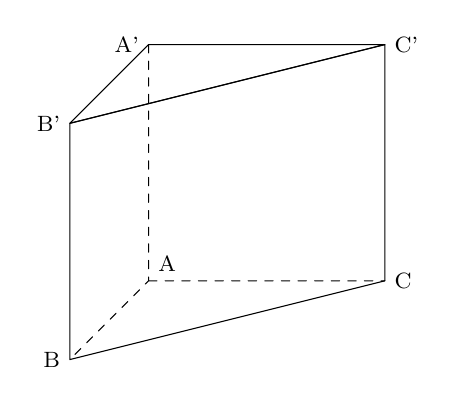
\begin{tikzpicture}[scale=1, font=\footnotesize, line join=round, line cap=round, >=stealth]
				\path
				(0,3) coordinate[label=left: A'] (A')
				(0,0) coordinate[label=above right: A] (A)
				(3,0) coordinate[label=right: C] (C)
				(3,3) coordinate[label=right: C'] (C')
				(-1,2) coordinate[label=left: B'] (B')
				(-1,-1) coordinate[label=left: B] (B)
				;
				\draw (A')--(B')--(C')--cycle;
				\draw (B)--(B')--(C')--(C)--cycle;
				\draw[dashed] (A')--(A)--(B) (A)--(C) ;		
			\end{tikzpicture}
		\end{center}
		Do $ABC.A'B'C'$ là lăng trụ đứng, nên ta có $\heva{&AC \perp AA' \\ & AB \perp AA'}$.\\
		Suy ra $\left[B,AA',C\right]=\widehat{CAB}$.\\
		Xét $\triangle ABC$ vuông tại $B$.\\
		Ta có $\tan CAB =\dfrac{BC}{AB}=\dfrac{a}{a\sqrt{3}}=\dfrac{\sqrt{3}}{3}$.\\
		Vậy  $\left[B,AA',C\right]=\widehat{CAB}=30^{\circ}$.
	}
\end{ex}

%%%==============EX_6============%%%
%\begin{ex}%[1H8N6-1]
%	Cho hình chóp $S.ABCD$ có đáy là hình chữ nhật và $SA\perp \left(ABCD\right)$. Góc giữa đường thẳng $SD$ và mặt phẳng $\left(ABCD\right)$ là góc nào sau đây?
%	\choice
%	{\True $\widehat{SDA}$}
%	{$\widehat{DSA}$}
%	{$\widehat{SCD}$}
%	{$\widehat{SDC}$}
%	\immini{	\loigiai{
%			$AD$ là hình chiếu của $SD$ lên mặt phẳng $\left(ABCD\right)$ $\Rightarrow \left(\widehat{SD,\left(ABCD\right)}\right)=\left(\widehat{SD,AD}\right)=\widehat{SDA}$.
%		}
%	}{\begin{tikzpicture}
%			\draw (3,0)--(2,-1)--(-1,-1);
%			\draw[dashed] (-1,-1)--(0,0)--(3,0);
%			\draw[dashed] (0,0)--(2,-1) (3,0)--(-1,-1);
%			\draw[dashed] (1,-.5)--(0,3)--(0,0);
%			\draw (-1,-1)--(0,3)--(2,-1)  (3,0)--(0,3);
%			\node[ left] at (0,0) {$A$} ;
%			\node[below left]at (-1,-1) {$B$} ;
%			\node[below right]at (3,0) {$D$} ;
%			\node[below right]at (2,-1) {$C$} ;
%			\node[left]at (0,3) {$S$} ;
%			\node[below]at (1,-.5) {$O$} ;
%	\end{tikzpicture}}
%\end{ex}

%%%==============EX_7============%%%
\begin{ex}%[1H8N6-2]
	Cho hình chóp $S.ABCD$ có đáy $ABCD$ là hình chữ nhật, tam giác $SAB$ đều và nằm trong mặt phẳng vuông góc với đáy. Gọi $H$, $K$ lần lượt là trung điểm của $AB$, $CD$. Góc phẳng nhị diện $\left[S, AB, K\right]$ là
	\choice
	{\True $\widehat{SHK}$}
	{$\widehat{SAK}$}
	{$\widehat{SAC}$}
	{$\widehat{SAD}$}
	\loigiai{\immini{
			Ta có $SH\perp AB$ và $KH\perp AB$, suy ra $\widehat{SHK}$ là góc phẳng nhị diện $\left[S, AB, K\right]$.}
		{
			\begin{tikzpicture}
				\path 
				(0,0) coordinate[label=left: A] (A)
				(5,0) coordinate[label=right: D] (D)
				(3,-2) coordinate[label=right: C] (C)
				(-2,-2) coordinate[label=left: B] (B)
				(-1,5) coordinate[label=left: S] (S)
				($(A)!0.5!(B)$) coordinate[label=left: H] (H)
				($(C)!0.5!(D)$) coordinate[label=right: K] (K);
				\draw (S)--(B)--(C)--(D)--cycle  (S)--(C);
				\draw[dashed] (S)--(H)--(K) (B)--(A)--(D)  (A)--(S) ;
			\end{tikzpicture}
		}
	}
\end{ex}

%%%==============EX_8============%%%
\begin{ex}%[1H8H6-1]
	Cho hình chóp $S.ABCD$ có đáy $\left(ABCD\right)$ là hình vuông cạnh $a$. Cạnh bên $SA$ vuông góc với mặt phẳng đáy $\left(ABCD\right)$. Góc giữa cạnh $SC$ và mặt phẳng $\left(SAD\right)$ là góc nào sau đây?
	\choice
	{$\widehat{SCA}$}
	{$\widehat{CSA}$}
	{$\widehat{SCD}$}
	{\True $\widehat{CSD}$}
	\loigiai{\immini{
			Ta có $SC\cap \left(SAD\right)=\left\{S\right\} (1)$.
			
			Mặt khác: $\heva{&CD\perp AD\\ &CD\perp SA \\ &AD\cap SA=\left\{A\right\}}$
			
			$\Rightarrow CD\perp \left(SAD\right)$, tức là $D$ là hình chiếu vuông góc của $C$ lên $\left(SAD\right) (2)$.
			
			Từ $(1)$, $(2)$ suy ra $SD$ là hình chiếu vuông góc của $SC$ lên $\left(SAD\right)$.
			
			Vậy góc giữa cạnh $SC$ và mặt phẳng $\left(SAD\right)$ là $\widehat{CSD}$.}{
			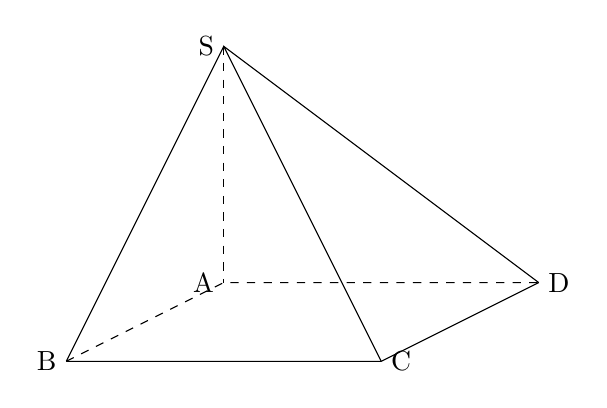
\begin{tikzpicture}
				\path
				(0,3) coordinate[label=left: S] (S)
				(0,0) coordinate[label=left: A] (A)
				(2,-1) coordinate[label=right: C] (C)
				(4,0) coordinate[label=right: D] (D)
				(-2,-1) coordinate[label=left: B] (B);
				\draw (D)--(C)--(B);
				\draw[dashed] (B)--(A)--(D);
				\draw[dashed] (S)--(A);
				\draw (B)--(S)--(C)  (D)--(S);
			\end{tikzpicture}
		}
	}
\end{ex}

%%%==============EX_9============%%%
\begin{ex}%[1H8V6-2]
	Cho hình chóp $S.ABCD$ có đáy $ABCD$ là hình thoi cạnh $a$ tâm $O$, $SO\perp \left(ABCD\right)$, $SO=\dfrac{a\sqrt{6}}{3}, OB=\dfrac{a\sqrt{3}}{3}$. Góc phẳng nhị diện $\left[A, BC, S\right]$ có số đo bằng
	\choice
	{$30^\circ$}
	{$45^\circ$}
	{\True $60^\circ$}
	{$90^\circ$}
	\loigiai{\immini{
			Gọi $H$ là hình chiếu của $S$ lên $BC$. 
			
			Ta có $SH\perp BC$ và $OH\perp BC$ suy ra $\widehat{SHO}$ là góc phẳng nhị diện $\left[A, BC, S\right]$.
			
			Ta có $OC=\sqrt{BC^2-OB^2}=\dfrac{a\sqrt{6}}{3}$
			
			 $\dfrac{1}{OH^2}=\dfrac{1}{OB^2}+\dfrac{1}{OC^2} \Rightarrow OH=\dfrac{a\sqrt{2}}{3}$.
			
			Trong tam giác vuông $SHO$ ta có
			
			 $\tan SHO=\dfrac{SO}{OH}=\sqrt{3}$.
			
			Suy ra $\widehat{SHO}=60^{\circ}$.}
		{
			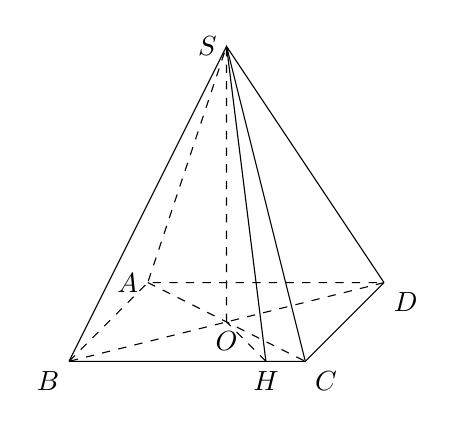
\begin{tikzpicture}
				\draw (3,0)--(2,-1)--(-1,-1);
				\draw[dashed] (-1,-1)--(0,0)--(3,0);
				\draw[dashed] (0,0)--(2,-1) (3,0)--(-1,-1);
				\draw[dashed] (1,-.5)--(1,3)--(0,0);
				\draw (-1,-1)--(1,3)--(2,-1)  (3,0)--(1,3);
				\draw (1,3)--(1.5,-1);
				\draw[dashed] (1.5,-1)--(1,-.5);
				\node[ left] at (0,0) {$A$} ;
				\node[below left]at (-1,-1) {$B$} ;
				\node[below right]at (3,0) {$D$} ;
				\node[below right]at (2,-1) {$C$} ;
				\node[left]at (1,3) {$S$} ;
				\node[below]at (1,-.5) {$O$} ;
				\node[below] at (1.5,-1) {$H$};
			\end{tikzpicture}
		}
	}
\end{ex}

%%%==============EX_10============%%%
\begin{ex}%[1H8H6-2]
	Cho hình chóp $S.ABC$ có đáy $ABC$ là tam giác vuông cân tại $A$, $SA\perp \left(ABC\right)$. Góc phẳng nhị diện $\left[B, SA, C\right]$ có số đo bằng
	\choice
	{$30^\circ$}
	{$45^\circ$}
	{$60^\circ$}
	{\True $90^\circ$}
	\loigiai{ \immini{
			Ta có $BA\perp SA$ và $CA\perp SA$ suy ra $\widehat{BAC}$ là góc phẳng nhị diện $\left[B, SA, C\right]$ và bằng $90^\circ$.}
		{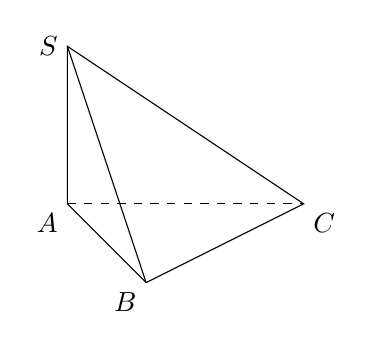
\begin{tikzpicture}
				\draw (0,0)--(1,-1)--(3,0)--(0,2)--cycle;
				\draw[dashed] (0,0)--(3,0);
				\draw (0,2)--(1,-1);
				\node[below left] at (0,0) {$A$} ;
				\node[below left]at (1,-1) {$B$} ;
				\node[below right]at (3,0) {$C$} ;
				\node[left]at (0,2) {$S$} ;
		\end{tikzpicture}}
	}
\end{ex}

%%%==============EX_11============%%%
%\begin{ex}%[1H8N6-1]
%	\immini{	Cho hình chóp tứ giác đều $S.ABCD$ có đáy là hình vuông tâm $O$. Góc giữa đường thẳng $SA$ và mặt phẳng $\left(SBD\right)$ là góc nào sau đây?
%		\choice
%		{\True $\widehat{ASO}$}
%		{$\widehat{ASB}$}
%		{$\widehat{ASD}$}
%		{$\widehat{AOS}$}
%		\loigiai{
%	}}{
%		\begin{tikzpicture}
%			\draw (3,0)--(2,-1)--(-1,-1);
%			\draw[dashed] (-1,-1)--(0,0)--(3,0);
%			\draw[dashed] (0,0)--(2,-1) (3,0)--(-1,-1);
%			\draw[dashed] (1,-.5)--(1,3)--(0,0);
%			\draw (-1,-1)--(1,3)--(2,-1)  (3,0)--(1,3);
%			\node[ left] at (0,0) {$A$} ;
%			\node[below left]at (-1,-1) {$B$} ;
%			\node[below right]at (3,0) {$D$} ;
%			\node[below right]at (2,-1) {$C$} ;
%			\node[left]at (1,3) {$S$} ;
%			\node[below]at (1,-.5) {$O$} ;
%		\end{tikzpicture}
%	}
%\end{ex}
%%%==============EX_12============%%%
\begin{ex}%[1H8H6-2]
	Cho hình chóp $S.ABC$ có $SA\perp \left(ABC\right)$. Gọi $H$ là hình chiếu của $A$ trên $BC$. Biết $\triangle ABC$ vuông tại $A$, $\widehat{ABC}=30^{\circ}$, $AC=a$, $SA=\dfrac{a\sqrt{3}}{2}$. Tính số đo góc nhị diện $\left[S,BC,A\right]$
	\choice
	{$30^\circ$}
	{\True $45^\circ$}
	{$60^\circ$}
	{$75^\circ$}
	\loigiai{\immini{
			Ta có $SA\perp \left(ABC\right)\Rightarrow SA\perp BC$.\\
			 Theo giả thiết $AH\perp BC$ $\Rightarrow BC\perp \left(SAH\right)$.\\
			$\Rightarrow \left[S,BC,A\right]=\widehat{SHA}$.\\
			Vì tam giác $ABC$ vuông tại $A$.\\ 
			nên ta có $\tan \widehat{ABC}=\dfrac{AC}{AB}$ $\Rightarrow AB=\dfrac{AC}{\tan 30^{\circ}}=a\sqrt{3}$.\\
			Khi đó:
			\begin{align*}
				\dfrac{1}{AH^2}&=\dfrac{1}{AB^2}+\dfrac{1}{AC^2}\\
				&=\dfrac{1}{3a^2}+\dfrac{1}{a^2}=\dfrac{4}{3a^2} \\
				\Rightarrow AH&=\dfrac{a\sqrt{3}}{2}.
			\end{align*} 
			Tam giác $SAH$ vuông tại $A$ có $SA=AH=\dfrac{a\sqrt{3}}{2}$ $\Rightarrow \widehat{SHA}=45^{\circ}$.}
		{
			\begin{tikzpicture}
				\path 
				(0,0) coordinate[label=left: A](A)
				(3,0) coordinate[label=right: C](C)
				(-2,-2) coordinate[label=left: B](B)
				(0,4) coordinate[label=above: S](S)
				($(B)!0.7!(C)$) coordinate[label=below: H](H)
				;
				\draw (S)--(B)--(C)--cycle (S)--(H) ;
				\draw[dashed] (B)--(A)--(S) (A)--(C) (A)--(H);
			\end{tikzpicture}
		}
	}
\end{ex} 
\Closesolutionfile{ans}
\indapan{6}{ans/ans-d2-lc}

\cauds
\Opensolutionfile{ans}[ans/ans-d2-ds]

%%%%==============Cau_EX1==============%%%
\begin{ex}%[1H8C6-6]
	Cho hình chóp $S.ABCD$ có đáy $ABCD$ là hình chữ nhật với $AB=a\sqrt{2}$,\hfill \, $AC=a\sqrt{3}$. Cạnh bên $SA=2a$ và vuông góc với mặt đáy $(ABCD)$. Khi đó, các mệnh đề sau \textbf{ĐÚNG} hay \textbf{SAI} ?
	\choiceTF
	{\True $AD\parallel (SBC)$}
	{Khoảng cách từ $D$ đến mặt phẳng $(SBC)$ bằng $\dfrac{a\sqrt{3}}{3}$}
	{\True Khoảng cách giữa hai đường thẳng $SD$, $AB$ bằng $\dfrac{2a\sqrt{5}}{5}$}
	{Thể tích khối chóp $S.ABCD$ bằng $\dfrac{\sqrt{2} a^3}{3}$}
	\loigiai{
		
		\begin{center}
					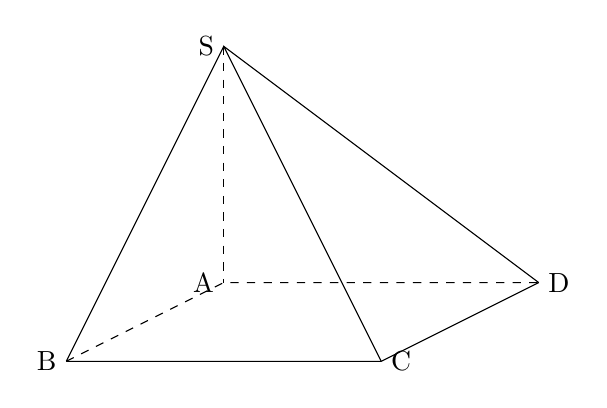
\begin{tikzpicture}
				\path
				(0,3) coordinate[label=left: S] (S)
				(0,0) coordinate[label=left: A] (A)
				(2,-1) coordinate[label=right: C] (C)
				(4,0) coordinate[label=right: D] (D)
				(-2,-1) coordinate[label=left: B] (B);
				\draw (D)--(C)--(B);
				\draw[dashed] (B)--(A)--(D);
				\draw[dashed] (S)--(A);
				\draw (B)--(S)--(C)  (D)--(S);
			\end{tikzpicture}
		\end{center}
		
		\begin{itemchoice}
			\itemch Đúng.
			
			Ta có $AD\parallel BC\Rightarrow AD\parallel (SBC)$
			\itemch Sai. 
			
			Ta có $ \mathrm{d}(D,(SBC))= \mathrm{d}(A,(SBC))$.
			
			Trong mặt phẳng $(SAB)$, kẻ $AH\perp SB$ tại $H$. \hfill{(1)}
			
			Ta có $\heva{&BC\perp AB \\ &BC\perp SA} \Rightarrow BC\perp (SAB)\Rightarrow AH\perp BC.$. \hfill{(2)}
			
			Từ $(1)$ và $(2)$ suy ra $AH\perp (SBC)$ hay $ \mathrm{d}(A,(SBC))=AH$.
			
			Tam giác $SAB$ vuông tại $A$ có đường cao $AH$ nên:
			\[\dfrac{1}{AH^2}=\dfrac{1}{SA^2}+\dfrac{1}{AB^2} \Rightarrow AH=\dfrac{SA\cdot AB}{\sqrt{SA^2+AB^2}}=\dfrac{2a\cdot a\sqrt{2}}{\sqrt{4a^2+2a^2}}=\dfrac{2a\sqrt{3}}{3}.\]
			Vậy $d(D,(SBC))=d(A,(SBC))=AH=\dfrac{2a\sqrt{3}}{3}$.
			\itemch Đúng.
			
			Trong mặt phẳng $(SAD)$, kẻ $AK\perp SD$ tại $K$.  \hfill{(3)}
			
			Ta có $\heva{&AB\perp SA \\ &AB\perp AD} \Rightarrow AB\perp (SAD)\Rightarrow AB\perp AK$.\hfill{(4)}
			
			Từ (3) và (4) suy ra $AK$ là đường vuông góc chung của hai đường thẳng chéo nhau $AB$, $SD$.
			
			Tam giác $ACD$ vuông tại $D$ nên $AD=\sqrt{AC^2-CD^2}=\sqrt{3a^2-2a^2}=a$.
			
			Tam giác $SAD$ vuông tại $A$ có đường cao $AK$ nên
			\[\dfrac{1}{AK^2}=\dfrac{1}{SA^2}+\dfrac{1}{AD^2} \Rightarrow AK=\dfrac{SA\cdot AD}{\sqrt{SA^2+AD^2}}=\dfrac{2a\cdot a}{\sqrt{4a^2+a^2}}=\dfrac{2a\sqrt{5}}{5}.\;\]
			
			Vậy $d(AB,SD)=AK=\dfrac{2a\sqrt{5}}{5}$.
			
			\itemch Sai.
			
			Diện tích đáy hình chóp là $S_{ABCD}=a\cdot a\sqrt{2}=a^2\sqrt{2}$.
			
			Thể tích khối chóp cần tìm là
			
			$V_{S.ABCD}=\dfrac{1}{3} SA\cdot S_{ABCD}=\dfrac{1}{3} \cdot 2a\cdot a^2\sqrt{2}=\dfrac{2\sqrt{2} a^3}{3} $ (đơn vị thể tích).
		\end{itemchoice}
	}
\end{ex}
%%%%==============HetCau_EX1==============%%%



%%%%==============Cau_EX2==============%%%
\begin{ex}%[1H8V6-5]
	Cho hình chóp $S.ABCD$ có đáy $ABCD$ là hình chữ nhật với $AB=2a$, $AD=a$. Hình chiếu của $S$ lên mặt phẳng $(ABCD)$ là trung điểm $H$ của $AB$ và $\widehat{SCH}=45^{\circ}$. Khi đó, các mệnh đề sau \textbf{ĐÚNG} hay \textbf{SAI} ?
	\choiceTF
	{\True $BC\perp (SAB)$}
	{\True $\mathrm{d}(H,(SBC))=\dfrac{a\sqrt{6}}{3}$}
	{Gọi $K$ là trung điểm $CD$ khi đó $CD\perp (SHK)$}
	{$\mathrm{d}(H,(SCD))=\dfrac{a\sqrt{6}}{2}$}
	\loigiai{
		
\begin{center}
					\begin{tikzpicture}
			\path
			(-1,3) coordinate[label=left: S] (S)
			(0,0) coordinate[label=above right: A] (A)
			(2,-1) coordinate[label=right: C] (C)
			(4,0) coordinate[label=right: D] (D)
			(-2,-1) coordinate[label=left: B] (B)
			($(A)!.5!(B)$) coordinate[label=below right: H] (H);
			\draw (D)--(C)--(B);
			\draw[dashed] (B)--(A)--(D);
			\draw[dashed] (S)--(A) (S)--(H);
			\draw (B)--(S)--(C)  (D)--(S);
		\end{tikzpicture}
\end{center}
		
		\begin{itemchoice}
			\itemch Đúng.
			
				Kẻ đường cao $HE$ trong tam giác $SBH$. \hfill{(1)} 

			
			Ta có $\heva{&BC\perp AB \\ &BC\perp SH(\text{ do } SH\perp (ABCD)} \Rightarrow BC\perp (SAB)\Rightarrow BC\perp HE$. \hfill{(2)}
			\itemch  Đúng.
			
				Từ (1) và (2) suy ra $HE\perp (SBC)$ hay $\mathrm{d}(H,(SBC))=HE$.
			
			Tam giác $BCH$ vuông tại $B$ có
			\[\begin{array}{ll} CH& {=\sqrt{BC^2+BH^2}} \\ {} & {=\sqrt{a^2+a^2}=a\sqrt{2}.} \end{array}\]
			
			Tam giác $SCH$ vuông tại $H$ có
			\[\tan \widehat{SCH}=\dfrac{SH}{CH} \Rightarrow SH=a\sqrt{2}.\;\]
			
			Tam giác $SBH$ vuông tại $H$ có đường cao $HE$ nên
			\[\begin{array}{ll} {\dfrac{1}{HE^2}} & {=\dfrac{1}{SH^2}+\dfrac{1}{BH^2}} \\[5pt] {\Rightarrow HE} & {=\dfrac{SH\cdot BH}{\sqrt{SH^2+BH^2}}} \\ {} & {=\dfrac{a\sqrt{2} \cdot a}{\sqrt{2a^2+a^2}}=\dfrac{a\sqrt{6}}{3}.} \end{array}\]
			
			Vậy $\mathrm{d}(H,(SBC))=HE=\dfrac{a\sqrt{6}}{3}$.
			\itemch Sai.
			
				Gọi $K$ là trung điểm $CD$ thì $HK$ là đường trung bình của hình chữ nhật $ABCD$ nên $HK\parallel BC\parallel AD\Rightarrow HK\perp CD$.
			
			Ta có $\heva{&CD\perp HK \\ &CD\perp SH} \Rightarrow CD\perp (SHK)$.
			\itemch Sai.
			
			
			Kẻ đường cao $HI$ của tam giác $SHK$.
			
			Ta có $\heva{&HI\perp SK \\ &HI\perp CD(\text{ do } CD\perp (SHK),HI\subset (SHK))} \Rightarrow HI\perp (SCD)$.
			
			Tam giác $SHK$ vuông tại $H$ có đường cao $HI$ nên
			\[\dfrac{1}{HI^2}=\dfrac{1}{SH^2}+\dfrac{1}{HK^2} \Rightarrow HI=\dfrac{SH\cdot HK}{\sqrt{SH^2+HK^2}}=\dfrac{a\sqrt{2} \cdot a}{\sqrt{2a^2+a^2}}=\dfrac{a\sqrt{6}}{3}.\]
			Vậy $d(H,(SCD))=HI=\dfrac{a\sqrt{6}}{3}$.
		\end{itemchoice}
	}
\end{ex}
%%%%==============HetCau_EX2==============%%%

%%%%==============Cau_EX3==============%%%
\begin{ex}%[1H8V6-5]
	Cho hình chóp đều $S.ABC$ có cạnh đáy bằng $a$, gọi $O$ là tâm của đáy và $SO=\dfrac{a\sqrt{3}}{3}$. Khi đó, các mệnh đề sau \textbf{ĐÚNG} hay \textbf{SAI} ?
	\choiceTF
	{$AO=\dfrac{a\sqrt{3}}{2}$}
	{\True $\mathrm{d}(O,SA)=\dfrac{a\sqrt{6}}{6}$}
	{\True Kẻ đường cao $AI$ của tam giác $ABC$, khi đó: $OI=\dfrac{a\sqrt{3}}{6}$}
	{$\mathrm{d}(O,(SBC))=\dfrac{a\sqrt{15}}{12}$}
	\loigiai{
		
		\begin{center}
			\begin{tikzpicture}
				\path
				(2.2,3) coordinate[label=left: S] (S)
				(0,0) coordinate[label=above left: A] (A)
				(5,0) coordinate[label=right: C] (C)
				(2,-2) coordinate[label=left: B] (B)
				($(A)!.5!(B)$) coordinate (H)
				($(C)!.5!(B)$) coordinate (K)
				($(C)!2/3!(H)$) coordinate[label=below: O] (O)
				;
				\draw (S)--(A)--(B)--(C) (S)--(B) (S)--(C);
				\draw[dashed] (A)--(C) (A)--(K) (C)--(H) (S)--(O);

			\end{tikzpicture}
		\end{center}
		
		\begin{itemchoice}
			\itemch Sai.
			
				Kẻ đường cao $AI$ của tam giác $ABC$, ta có $O$ thuộc $AI$.
			
			Trong mặt phẳng $(SAI)$, dựng $OH\perp SA$ tại $H\Rightarrow \mathrm{d}(O,SA)=OH$.
			
			Tam giác $ABC$ đều cạnh $a$ nên $AO=\dfrac{2}{3} AI=\dfrac{2}{3} \cdot \dfrac{a\sqrt{3}}{2}=\dfrac{a\sqrt{3}}{3}=SO$. 
			\itemch Đúng.
			
			 Tam giác $SAO$ vuông cân tại $O$ nên $OH=\dfrac{SA}{2}=\dfrac{\dfrac{a\sqrt{3}}{3} \cdot
				 \sqrt{2}}{2}=\dfrac{a\sqrt{6}}{6}$.
				 
			Vậy $\mathrm{d}(O,SA)=OH=\dfrac{a\sqrt{6}}{6}.$
			\itemch Đúng.
			
				Ta có $OI=\dfrac{AI}{3}=\dfrac{\dfrac{a\sqrt{3}}{2}}{3}=\dfrac{a\sqrt{3}}{6}$.
			
			\itemch Sai.
			
			Ta xét khoảng cách từ $O$ đến mặt bên $(SBC)$.
			
			Kẻ đường cao $OK$ của tam giác $SOI$. \hfill{(1)}
			
			Ta có $\heva{&BC\perp SO(\text{ do } SO\perp (ABC)) \\& BC\perp AI} \Rightarrow BC\perp (SAI)\Rightarrow BC\perp OK$.\hfill{(2)}
			
			Từ $(1)$ và $(2)$ suy ra $OK\perp (SBC)$ hay $OK=d(O,(SBC))$.
			
			
			Tam giác $SOI$ vuông tại $O$ có đường cao $OK$ nên
			\[\dfrac{1}{OK^2}=\dfrac{1}{SO^2}+\dfrac{1}{OI^2} \Rightarrow OK=\dfrac{SO\cdot OI}{\sqrt{SO^2+OI^2}}=\dfrac{\dfrac{a\sqrt{3}}{3} \cdot \dfrac{a\sqrt{3}}{6}}{\sqrt{\dfrac{3a^2}{9}+\dfrac{3a^2}{36}}}=\dfrac{a\sqrt{15}}{15}\]
			Vậy $\mathrm{d}(O,(SBC))=OK=\dfrac{a\sqrt{15}}{15}$.
		\end{itemchoice}
	}
\end{ex}
%%%%==============HetCau_EX3==============%%%


%%%%==============Cau_EX4==============%%%
\begin{ex}%[1H8V6-5]
	Cho hình lăng trụ tam giác đều $ABC\cdot A' B' C'$ có cạnh đáy bằng $2a$, khoảng cách từ điểm $A'$ đến mặt phẳng $\left(AB' C' \right)$ bằng $\dfrac{a\sqrt{3}}{2}$. Khi đó, các mệnh đề sau \textbf{ĐÚNG} hay \textbf{SAI}?
	\choiceTF
	{\True Trong mặt phẳng $\left(A' B' C' \right)$, kẻ $A' H\perp B' C'$ tại $H$. Khi đó: $B'C'\perp (AA'H)$}
	{\True $\mathrm{d}\left((ABC),\left(A' B' C' \right)\right)=a$}
	{ Diện tích đáy của lăng trụ là $a^2\sqrt{5}$}
	{\True Thể tích khối lăng trụ là $a^3\sqrt{3}$}
	\loigiai{
		
				\begin{center}
			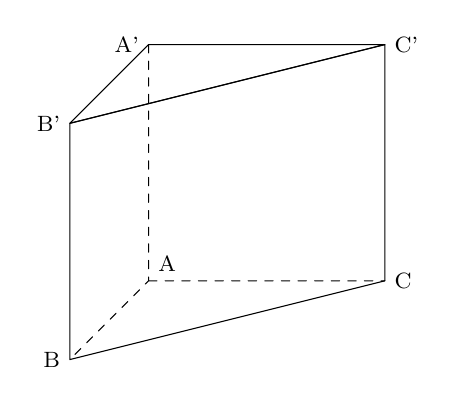
\begin{tikzpicture}[scale=1, font=\footnotesize, line join=round, line cap=round, >=stealth]
				\path
				(0,3) coordinate[label=left: A'] (A')
				(0,0) coordinate[label=above right: A] (A)
				(3,0) coordinate[label=right: C] (C)
				(3,3) coordinate[label=right: C'] (C')
				(-1,2) coordinate[label=left: B'] (B')
				(-1,-1) coordinate[label=left: B] (B)
;
				\draw (A')--(B')--(C')--cycle;
				\draw (B)--(B')--(C')--(C)--cycle;
				\draw[dashed] (A')--(A)--(B) (A)--(C) ;		
			\end{tikzpicture}
		\end{center}
		
		\begin{itemchoice}
			\itemch Đúng.
			
			Trong mặt phẳng $\left(A' B' C' \right)$, kẻ $A' H\perp B' C'$ tại $H$.
			
			Trong mặt phẳng $\left(AA' H\right)$, kẻ $A' K\perp AH$ tại $K$. \hfill{(1)}
			
			Ta có $\heva{&B'C'\perp A'H \\ &B'C'\perp AA'(do AA'\perp (A'B'C'))} \Rightarrow B'C'\perp (AA'H)$.
			\itemch Đúng.
			
				Ta có $ A'K\perp B'C'$. \hfill{(2)}
				
			Từ $(1)$ và $(2)$ suy ra $A' K\perp \left(AB' C' \right)$ hay $\mathrm{d}\left(A', \left(AB' C' \right)\right)=A' K=\dfrac{a\sqrt{3}}{2}$.
			
			Tam giác $A' B' C'$ đều có đường cao $A' H=\dfrac{2a\cdot \sqrt{3}}{2}=a\sqrt{3}$.
			
			Tam giác $AA' H$ vuông tại $A'$ có đường cao $A' K$ nên
			\[\dfrac{1}{A' K^2}=\dfrac{1}{A' H^2}+\dfrac{1}{A' A^2} \Rightarrow \dfrac{1}{\dfrac{3a^2}{4}}=\dfrac{1}{3a^2}+\dfrac{1}{A' A^2} \Rightarrow A' A=a.\]
			\itemch Sai.
			
			 Hai mặt đáy lăng trụ song song với nhau và có khoảng cách là
			 
			  $\mathrm{d}\left((ABC),\left(A' B' C' \right)\right)=AA'=a.\;$
			
			Diện tích đáy của lăng trụ (đáy là tam giác đều) là $S_{\Delta A' B' C'}=\dfrac{(2a)^2\sqrt{3}}{4}=a^2\sqrt{3}$
			\itemch Đúng.
			
				Thể tích khối lăng trụ là: $V=AA' \cdot S_{\Delta A' B' C'}=a\cdot a^2\sqrt{3}=a^3\sqrt{3}$ (đơn vị thể tích).
		\end{itemchoice}
	}
\end{ex}
%%%%==============HetCau_EX4==============%%%

\Closesolutionfile{ans}
\indapan{3}{ans/ans-d2-ds}

\Opensolutionfile{ans}[ans/ans-de2-kq]
\caukq
%%%==============BT_1==============%%%
\begin{bt}%[1H8H6-1]
	Cho hình chóp $S.ABC$ có đáy là tam giác đều cạnh $a$ và $SB\perp (ABC)$ và $SB=4a$. Tính góc giữa đường thẳng $SC$ và mặt phẳng $(SAB)$? (đơn vị đo góc là độ, làm tròn đến hàng phần chục)
	\shortans{$12{,}1$}
	\loigiai{
		
				\begin{center}
			\begin{tikzpicture}
				\path
				(0,3) coordinate[label=left: S] (S)
				(0,0) coordinate[label=above left: B] (B)
				(5,0) coordinate[label=right: C] (C)
				(2,-2) coordinate[label=left: A] (A)
				($(A)!.5!(B)$) coordinate (H)
				($(C)!.5!(B)$) coordinate (K)
				;
				\draw (S)--(A)--(C)--cycle (S)--(B)--(A);
				\draw[dashed] (B)--(C);
				
			\end{tikzpicture}
		\end{center}
		Kẻ $CI\perp AB\Rightarrow I$ là trung điểm $AB$.\\
		Ta có $\heva{&CI\perp AB \\ &CI\perp SB} \Rightarrow CI\perp (SAB)$ tại $I$ và $SC$ cắt mp $(SAB)$ tại $S$.\\
		$\Rightarrow SI$ là hình chiếu của $SC$ trên mp $(SAB)$.\\
		$\Rightarrow (SC,(SAB))=(SC,SI)=\widehat{CSI}$
		Ta có $IC=\dfrac{a\sqrt{3}}{2}$.\\
		Ta có $SC=\sqrt{SB^2+BC^2}=\sqrt{(4a)^2+a^2}=\sqrt{17} a$.\\
		Xét $\triangle SCI$ vuông tại $I$: $\sin \widehat{CSI}=\dfrac{CI}{SC}=\dfrac{\dfrac{a\sqrt{3}}{2}}{\sqrt{17} a}=\dfrac{\sqrt{51}}{34} \Rightarrow \widehat{CSI}\approx 12,1^\circ$.\\
		Vậy $(SC,(SAB))\approx 12,1^{\circ}$.
	}
\end{bt}

%%%==============BT_2==============%%%
\begin{bt}%[1H8H6-2]
	Cho hình chóp $S.ABCD$ có đáy là hình vuông cạnh $2a$ và $SC\perp (ABCD)$ và $SC=3a$. Góc phẳng nhị diện $[B,SA,C]$ có số đo là? (đơn vị đo góc là độ, làm tròn đến hàng đơn vị)
	\shortans{$54$}
	\loigiai{
		
				\begin{center}
			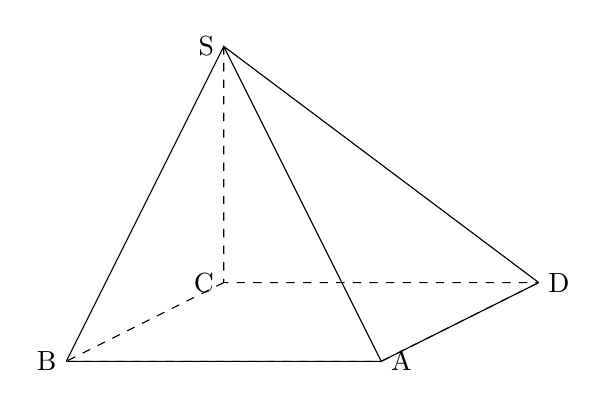
\begin{tikzpicture}
				\path
				(0,3) coordinate[label=left: S] (S)
				(0,0) coordinate[label=left: C] (C)
				(2,-1) coordinate[label=right: A] (A)
				(4,0) coordinate[label=right: D] (D)
				(-2,-1) coordinate[label=left: B] (B);
				\draw (D)--(A)--(B);
				\draw[dashed] (B)--(A)--(D);
				\draw[dashed] (S)--(C)--(D) (C)--(B) ;
				\draw (B)--(S)--(A)  (D)--(S);
			\end{tikzpicture}
		\end{center}
		Ta có $\heva{&BO\perp SA\\ &BO\perp AC} \Rightarrow BO\perp (SAC)$.\\
		Ta có $\heva{&(SBA)\cap (SAC)=SA \\ &\text{Trong } (SAC),OI\perp SA  \\ & \text{Trong }  (SBA),BI\perp SA} \Rightarrow [B,SA,C]=[B,SA,O]=\widehat{BIO}$.\\
		Ta có $\triangle IAO \backsim \triangle CAS\Rightarrow \dfrac{OI}{SC}=\dfrac{OA}{SA}$\\
		$ \Rightarrow OI=\dfrac{OA\cdot SC}{SA}=\dfrac{\sqrt{2} a.3a}{\sqrt{(3a)^2+(2\sqrt{2} a)^2}}=\dfrac{3\sqrt{34}}{17} a$.\\
		Xét $\triangle BOI$ vuông tại $O:\tan \widehat{BIO}=\dfrac{BO}{IO}=\dfrac{a\sqrt{2}}{\dfrac{3\sqrt{34}}{17} a}=\dfrac{\sqrt{17}}{3}$
		$ \Rightarrow \widehat{BIO}\approx 54^{\circ}.$
	}
\end{bt}

%%%==============BT_3==============%%%
\begin{bt}%[1H8H6-2]
	Cho hình lăng trụ đứng $ABC\cdot A' B' C'$ có đáy là tam giác vuông cân tại $B$. $AC=2a$ và $A' B=3a$. Tính góc phẳng nhị diện $\left[B', AC,B\right]$? (đơn vị đo góc là độ, làm tròn đến hàng phần chục)
	\shortans{$69{,}3$}
	\loigiai{
		
					\begin{center}
			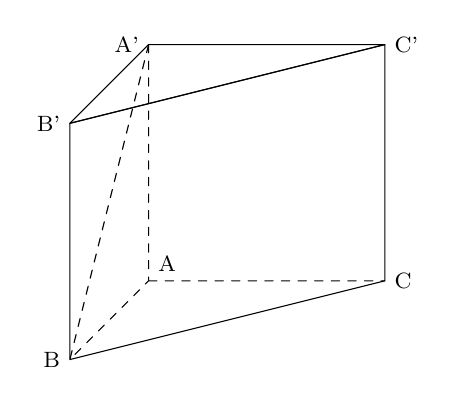
\begin{tikzpicture}[scale=1, font=\footnotesize, line join=round, line cap=round, >=stealth]
				\path
				(0,3) coordinate[label=left: A'] (A')
				(0,0) coordinate[label=above right: A] (A)
				(3,0) coordinate[label=right: C] (C)
				(3,3) coordinate[label=right: C'] (C')
				(-1,2) coordinate[label=left: B'] (B')
				(-1,-1) coordinate[label=left: B] (B)
				;
				\draw (A')--(B')--(C')--cycle;
				\draw (B)--(B')--(C')--(C)--cycle; 
				\draw[dashed] (A')--(A)--(B) (A)--(C)  (A')--(B);		
			\end{tikzpicture}
		\end{center}
		
		Ta có $BI=\dfrac{AC}{2}=a$, $B' B=\sqrt{(3a)^2-(a\sqrt{2})^2}=\sqrt{7} a$.\\
		Xét $\Delta BB' I$ vuông tại $B:\tan \widehat{B' IB}=\dfrac{B' B}{BI}=\dfrac{\sqrt{7} a}{a}=\sqrt{7} \Rightarrow \widehat{B' IB}\approx 69,3^{\circ}$.
	}
\end{bt}

%%%==============BT_4==============%%%
\begin{bt}%[1H8H6-2]
	Cho hình chóp $S.ABC$ có đáy $ABC$ là tam giác vuông tại $A,\widehat{ABC}=60^{\circ}$, tam giác $SBC$ là tam giác đều có bằng cạnh $2a$ và nằm trong mặt phẳng vuông với đáy. Gọi $\varphi$ là góc phẳng nhị diện $[S,AC,B]$. Tính tan $\varphi$? (làm tròn đến hàng phần trăm)
	\shortans{$3{,}46$}
	\loigiai{
				\begin{center}
			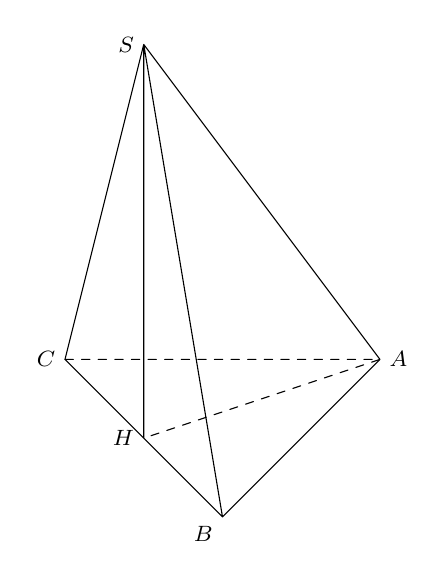
\begin{tikzpicture}[scale=1, font=\footnotesize, line join=round, line cap=round, >=stealth]
				\draw[dashed] (0,0)--(4,0)--(1,-1);
				\draw(0,0)--(2,-2)--(4,0)--(1,4)--(1,-1) (0,0)--(1,4)--(2,-2);
				\node[right] at (4,0) {$A$} ;
				\node[left] at (0,0) {$C$} ;
				\node[below left]at (2,-2) {$B$} ;
				\node[left]at (1,4) {$S$} ;
				\node[left]at (1,-1) {$H$} ;
			\end{tikzpicture}
		\end{center}
		Gọi $H$ là trung điểm của $BC$, suy ra $SH\perp BC\Rightarrow SH\perp (ABC)$.\\
		Gọi $K$ là trung điểm $AC$, suy ra $HK\parallel AB$ nên $HK\perp AC$.\\
		Ta có $\heva{&AC\perp HK\\ &AC\perp SH} \Rightarrow AC\perp (SHK)\Rightarrow AC\perp SK$\\
		Do đó $[S,AC,B]=(SK,HK)=\widehat{SKH}$.\\
		Tam giác vuông $ABC$, có $AB=BC\cdot \cos \widehat{ABC}=a$
		$\Rightarrow HK=\dfrac{1}{2} AB=\dfrac{a}{2}
		$.\\
		Tam giác vuông $SHK$, có $\tan \widehat{SKH}=\dfrac{SH}{HK}=2\sqrt{3}$.
	}
\end{bt}

%%%==============BT_5==============%%%
\begin{bt}%[1H8H6-1]
	Cho hình chóp $S.ABC$ có đáy là tam giác đều cạnh $a$, $SB\perp (ABC)$ và $SB=4a$. Tính góc giữa đường thẳng $SC$ và mặt phẳng $(SAB)$? (đơn vị đo góc là độ, làm tròn đến hàng phần chục)
	\shortans{ $12{,}1$}
	\loigiai{
		
					\begin{center}
			\begin{tikzpicture}
				\path
				(0,3) coordinate[label=left: S] (S)
				(0,0) coordinate[label=above left: B] (B)
				(5,0) coordinate[label=right: C] (C)
				(2,-2) coordinate[label=left: A] (A)
				($(A)!.5!(B)$) coordinate (H)
				($(C)!.5!(B)$) coordinate (K)
				;
				\draw (S)--(A)--(C)--cycle (S)--(B)--(A);
				\draw[dashed] (B)--(C);
				
			\end{tikzpicture}
		\end{center}
		Kẻ $CI\perp AB\Rightarrow$ $I$ là trung điểm $AB$.\\
		Ta có $\heva {&CI\perp AB \\ &CI\perp SB} \Rightarrow CI\perp (SAB)$ tại $I$ và $SC$ cắt $mp(SAB)$ tại $S$.\\
		$\Rightarrow$ $SI$ là hình chiếu của $SC$ trên $mp(SAB)$.\\
		$\Rightarrow (SC,(SAB))=(SC,SI)=\widehat{CSI}
		$
		Ta có $IC=\dfrac{a\sqrt{3}}{2}$.\\
		Ta có $SC=\sqrt{SB^2+BC^2}=\sqrt{(4a)^2+a^2}=\sqrt{17} a$.\\
		Xét $\triangle SCI$ vuông tại $I$: $\sin \widehat{CSI}=\dfrac{CI}{SC}=\dfrac{\dfrac{a\sqrt{3}}{2}}{\sqrt{17} a}=\dfrac{\sqrt{51}}{34} \Rightarrow \widehat{CSI}\approx 12,1^{\circ}$.\\
		Vậy $(SC,(SAB))\approx 12{,}1^{\circ}$.
	}
\end{bt}

%%%==============BT_6==============%%%
\begin{bt}%[1H8H6-2]
	Cho hình chóp $S.ABCD$ có đáy là hình vuông cạnh $2a$, $SC\perp (ABCD)$ và $SC=3a$. Tính góc phẳng nhị diện $[B,SA,C]$? (đơn vị đo góc là độ, làm tròn đến hàng đơn vị)
	\shortans{$54$}
	\loigiai{
		
						\begin{center}
			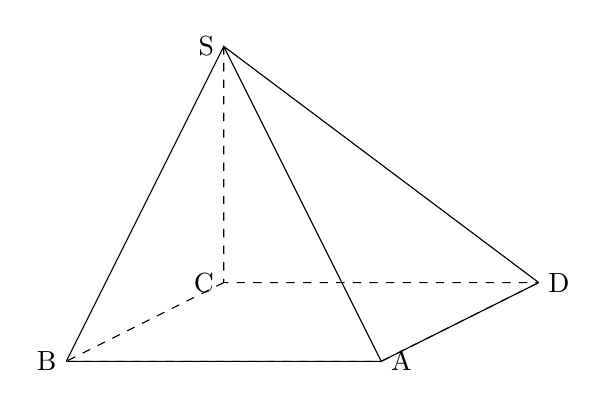
\begin{tikzpicture}
				\path
				(0,3) coordinate[label=left: S] (S)
				(0,0) coordinate[label=left: C] (C)
				(2,-1) coordinate[label=right: A] (A)
				(4,0) coordinate[label=right: D] (D)
				(-2,-1) coordinate[label=left: B] (B);
				\draw (D)--(A)--(B);
				\draw[dashed] (B)--(A)--(D);
				\draw[dashed] (S)--(C)--(D) (C)--(B) ;
				\draw (B)--(S)--(A)  (D)--(S);
			\end{tikzpicture}
		\end{center}
		Ta có $\heva{&BO\perp SC \\ &BO\perp AC} \Rightarrow BO\perp (SAC)$.\\
		Ta có $\heva{&(SBA)\cap (SAC)=SA \\ &\text{Trong }(SAC),OI\perp SA \\ &\text{Trong }(SBA),BI\perp SA} \Rightarrow [B,SA,C]=[B,SA,O]=\widehat{BIO}$.\\
		Ta có $\triangle IAO\sim \triangle CAS\Rightarrow \dfrac{OI}{SC}=\dfrac{OA}{SA} $\\
		$\Rightarrow OI=\dfrac{OA\cdot SC}{SA}=\dfrac{\sqrt{2} a\cdot 3a}{\sqrt{(3a)^2+(2\sqrt{2} a)^2}}=\dfrac{3\sqrt{34}}{17} a$.\\
		Xét $\triangle BOI$ vuông tại O: $\tan \widehat{BIO}=\dfrac{BO}{IO}=\dfrac{a\sqrt{2}}{\dfrac{3\sqrt{34}}{17} a}=\dfrac{\sqrt{17}}{3} \Rightarrow \widehat{BIO}\approx 54^{\circ}$.
	}
\end{bt}



\Closesolutionfile{ans}
\indapan{6}{ans/ans-de2-kq}